\documentclass[11pt]{article}

\usepackage{comment} % enables the use of multi-line comments (\ifx \fi) 
\usepackage[a4paper,margin=1cm]{geometry}
\usepackage[utf8]{inputenc}
\usepackage[ngerman]{isodate}
\usepackage{gensymb}
\usepackage{graphicx}
\usepackage{booktabs}% http://ctan.org/pkg/booktabs
\usepackage{tabularx}
\usepackage{multirow}
\usepackage{ltablex} % Longtables with tabularx
\usepackage[x11names,table]{xcolor}
\usepackage{amsmath}
\usepackage{amssymb}
\usepackage{amsthm}
\usepackage{array}
\usepackage{wrapfig}
\usepackage{subcaption}
\usepackage{csquotes}
\usepackage{lscape}
\usepackage{geometry}
\usepackage{multicol}
\usepackage{bm}
\usepackage{enumitem}
\usepackage{hyperref}
\usepackage{mdframed}
\usepackage{scalerel}
\usepackage{stackengine}
\usepackage{mathtools}
\usepackage{pdfpages}

% Code highlighting
\usepackage{minted}
\surroundwithmdframed{minted}

% Be able to caption equations and float them in place
\usepackage{float}

% Bibliography & citing
\usepackage[
	backend=biber,
	style=apa,
	bibstyle=apa,
	citestyle=apa,
	autolang=langname,
	sortlocale=en_UK
]{biblatex}
\addbibresource{Bibliography.bib}
% print the whole bibliography
\nocite{*}

\newmdtheoremenv{theorem}{Theorem}

\theoremstyle{definition}
\newmdtheoremenv{definition}{Definition}[section]


\geometry{a4paper, margin=2.4cm}

\newcommand\equalhat{\mathrel{\stackon[1.5pt]{=}{\stretchto{\scalerel*[\widthof{=}]{\wedge}{\rule{1ex}{3ex}}}{0.5ex}}}}
\newcommand\defeq{\mathrel{\overset{\makebox[0pt]{\mbox{\normalfont\tiny def}}}{=}}}
\newcolumntype{C}{>{\centering\arraybackslash}X}

\newcommand*\samplemean[1]{\overline{#1}}
\newcommand*\ev[1]{\mathrel{\text{E}\left[#1\right]}}
\newcommand*\R{\mathbb{R}}
\newcommand*\Z{\mathbb{Z}}
\newcommand*\N[1]{\mathcal{N}\left(#1\right)}
\newcommand*\Likelihood{\mathcal{L}}
\newcommand*\diff{\mathop{}\!\mathrm{d}}
\newcommand*\Diff[1]{\mathop{}\!\mathrm{d^#1}}
\newcommand*\Exp[1]{\mathop{\text{Exp}}\left(#1\right)}
\newcommand*\Cov[1]{\mathop{\text{Cov}}\left(#1\right)}
\newcommand*\Cor[1]{\mathop{\text{Cor}}\left(#1\right)}
\newcommand*\Var[1]{\mathop{\text{Var}}\left(#1\right)}

\DeclarePairedDelimiter\abs{\lvert}{\rvert}
\DeclarePairedDelimiter\norm{\lVert}{\rVert}

\setcounter{tocdepth}{3}
\setcounter{secnumdepth}{3}

\graphicspath{{./img/}}

\begin{document}
	
\title{Ethics HS21}
\author{Pascal Baumann\\pascal.baumann@stud.hslu.ch}
\maketitle

For errors or improvement raise an issue or make a pull request on the \href{https://github.com/KilnOfTheSecondFlame/mse_summaries}{github repository}.

\tableofcontents
\newpage

\section{Introduction}

\subsection{The Need for Ethics}
The fundamental question of ethics is \textquotedblleft What should I do\textquotedblright. This question reflects freedom and commitment, but an individual should also
\begin{itemize}[label=-, nosep]
	\item be good
	\item behave well
	\item strive for good conditions
\end{itemize}

\noindent
Ethics can help in this aspect in the following way
\begin{itemize}[nosep]
	\item As a guideline for human action
	\item Ethical debates are advice for laws
\end{itemize}

\begin{figure}[tbh]
	\centering
	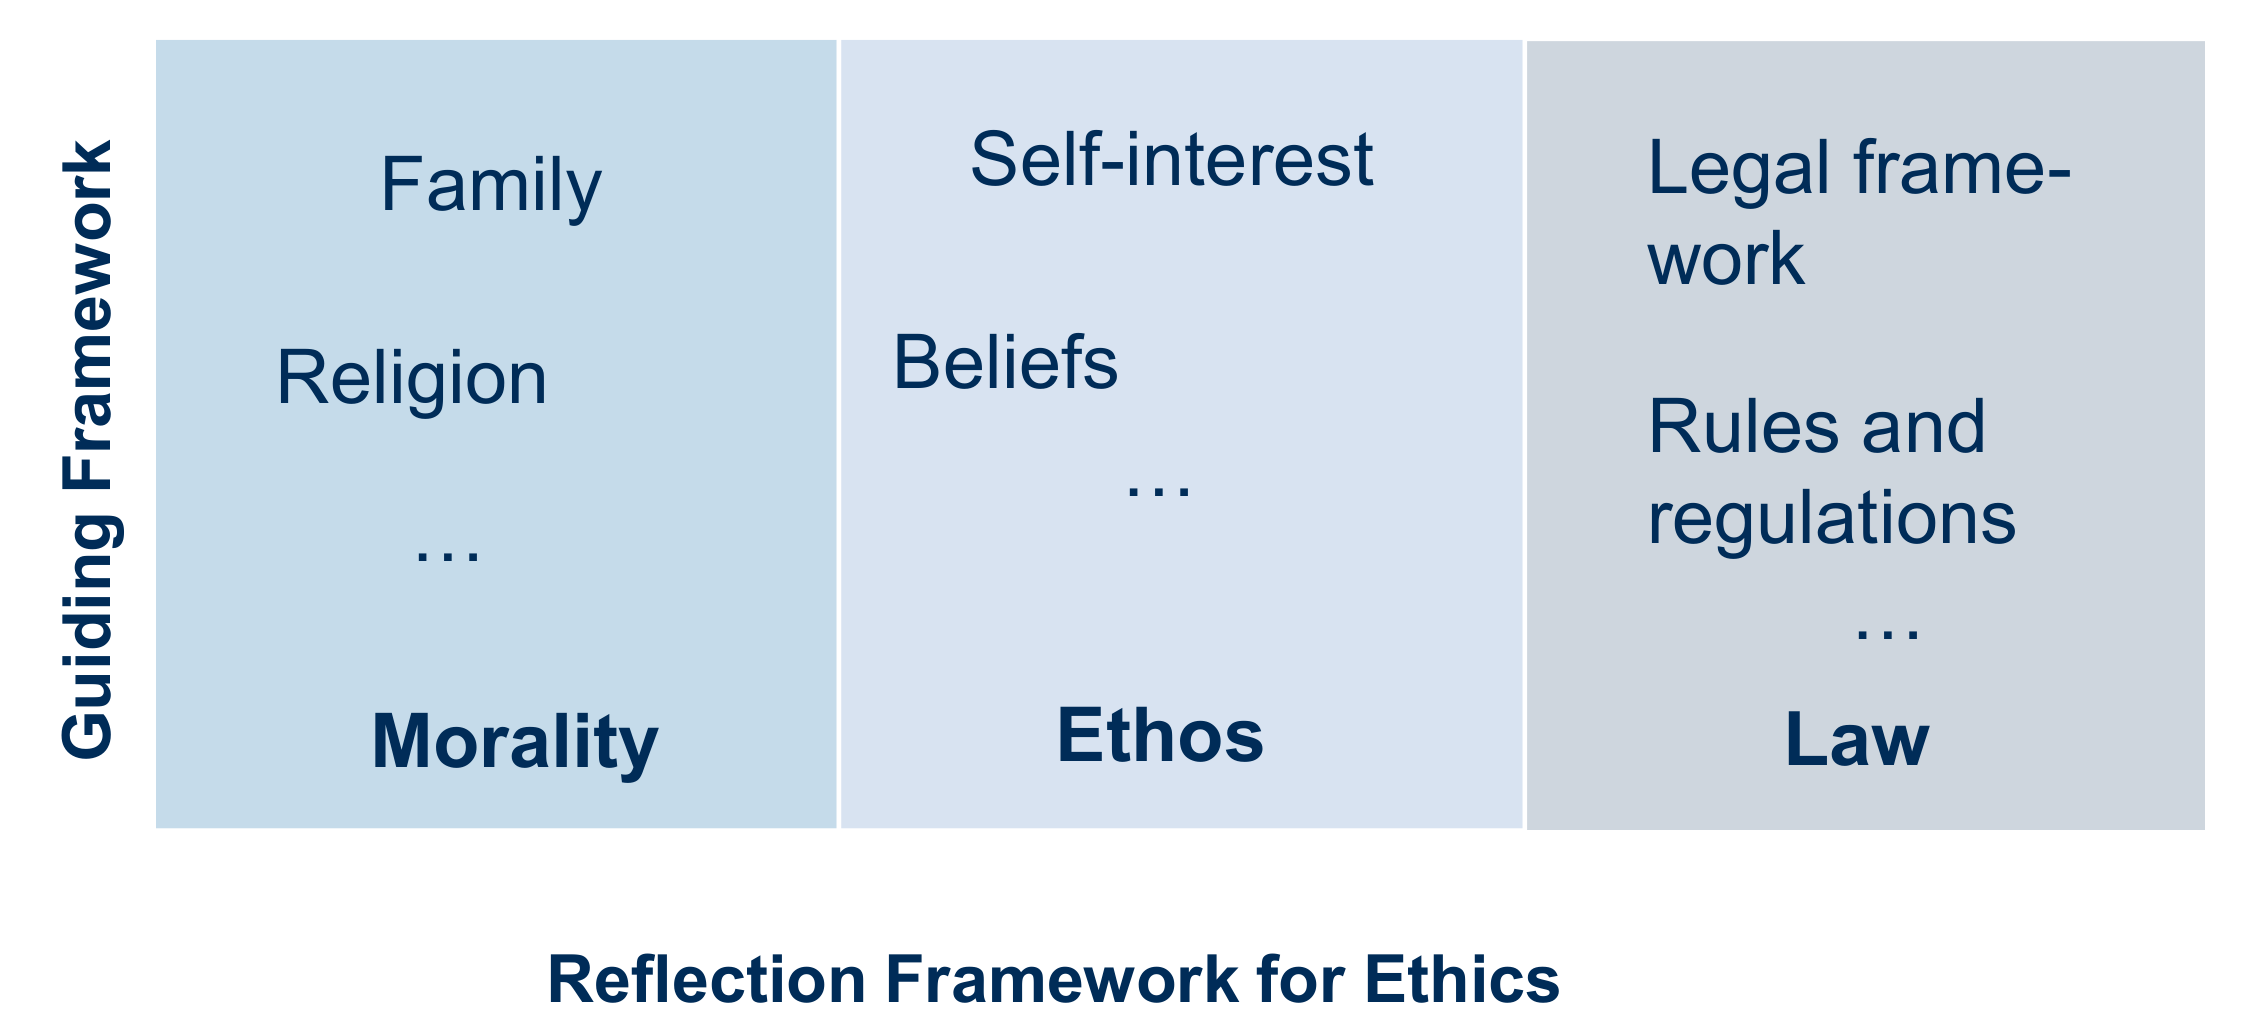
\includegraphics[width=0.8\linewidth]{img/ethics_frame}
	\caption{The different frames an ethical question can arise in}
	\label{fig:ethicsframe}
\end{figure}

\begin{figure}[tbh]
	\centering
	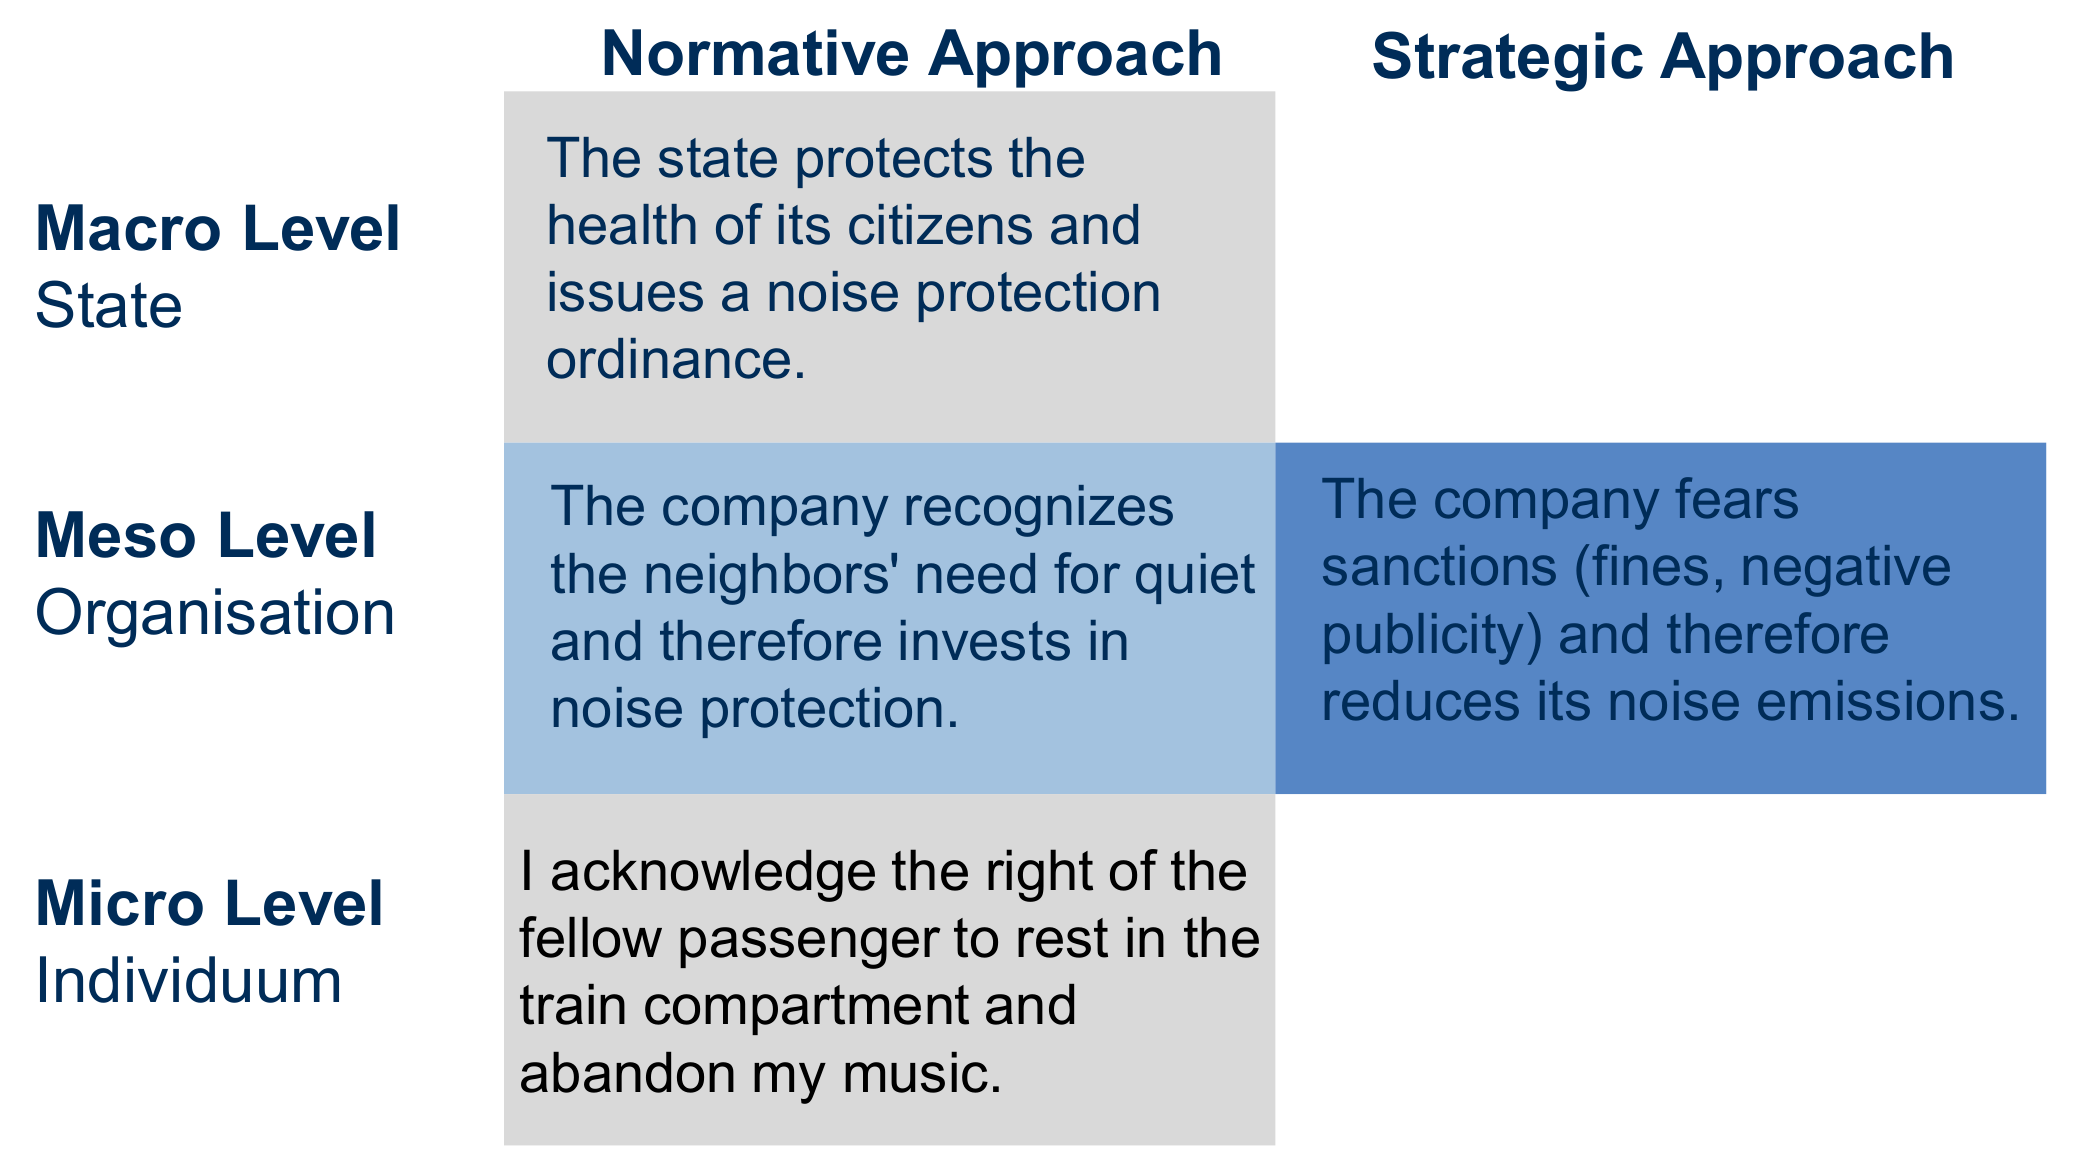
\includegraphics[width=0.6\linewidth]{img/ethics_approach}
	\caption{Normative and Strategic Approaches broken down into Macro-, Meso- and Micro-Level}
	\label{fig:ethicsapproach}
\end{figure}

\begin{definition}
	\textbf{Morality} is what at a certain time in a certain society is generally considered good and desirable or evil and forbidden as an action, condition, or attitude is collectively called the prevailing morality \parencite{gobel2013unternehmensethik}.
	
	\vspace*{1em}
	\noindent
	Morality only means that a system of norms claims to be valid, not that it is justified.
\end{definition}

\begin{definition}
	\textbf{Law} can be understood as a system of positive coercive norms applying to individuals, including sanctions associated with them.
\end{definition}

\begin{definition}
	\textbf{Ethos} refers to a subject who recognizes a certain morality as a requirement for his or her actions and to actions that are consistently marked by recognition.
\end{definition}

\begin{center}
	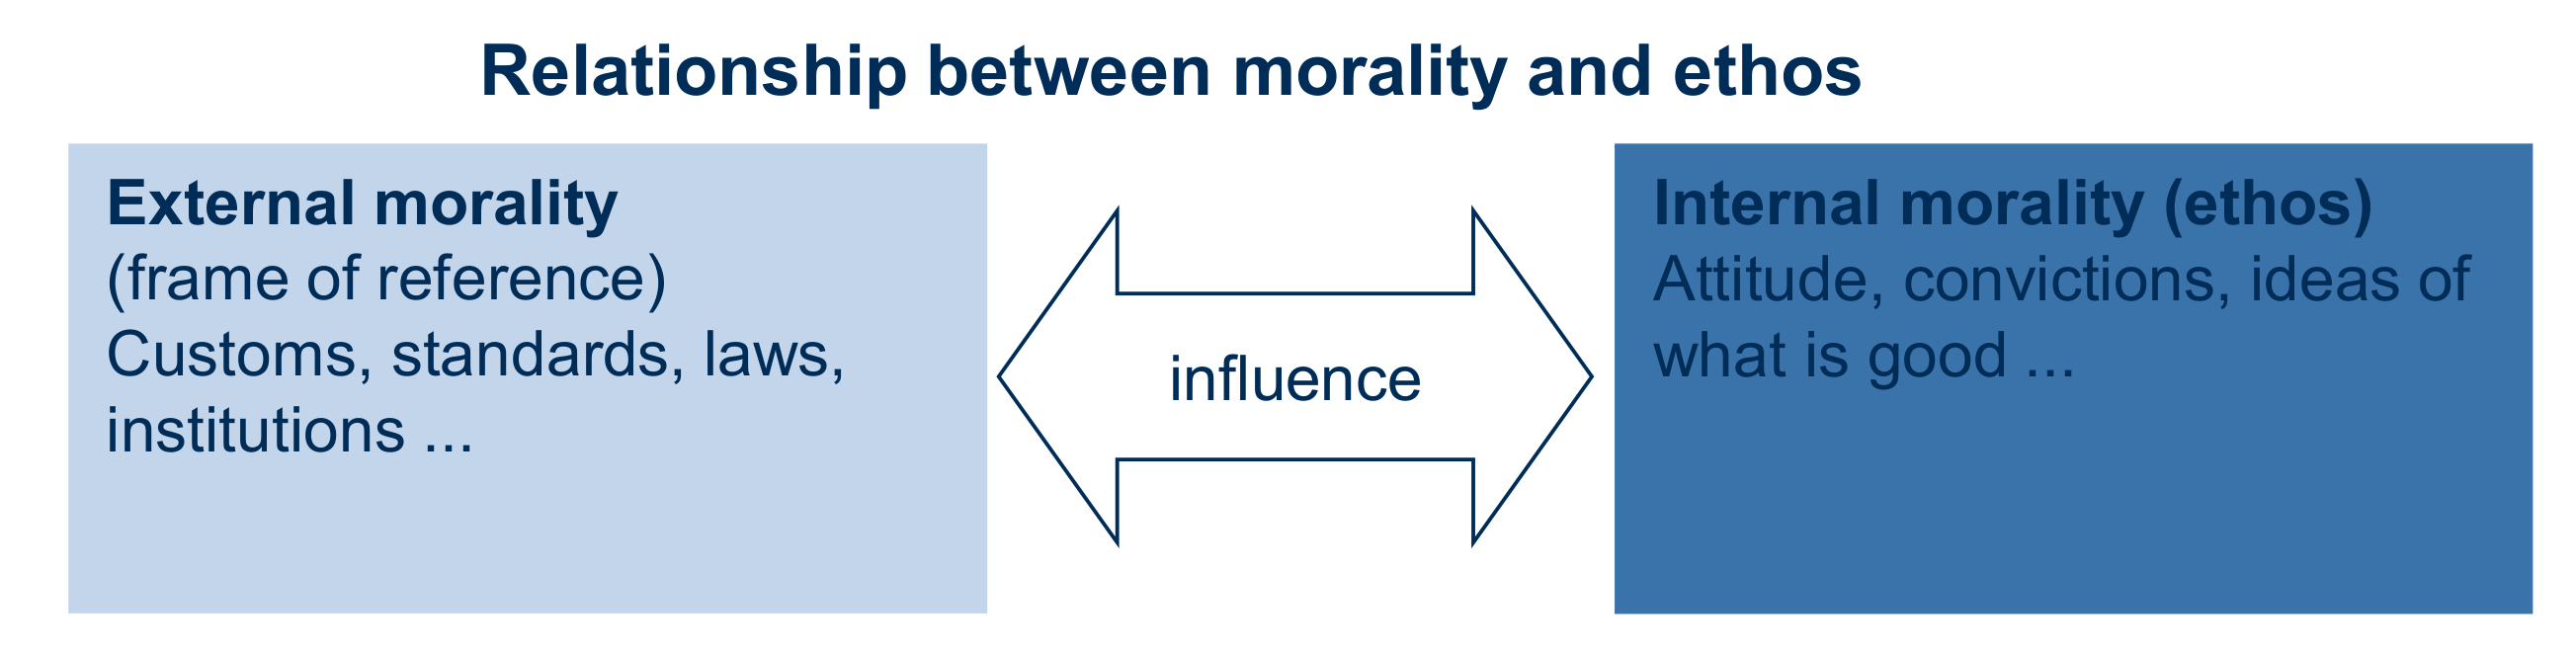
\includegraphics[width=0.8\linewidth]{img/ethos}
\end{center}

\begin{definition}
	\textbf{Ethics} in general can be described as the teaching or the science of morals and ethos.
\end{definition}

Ethics analyses the answers provided by different forms of morality to questions on what one should do, one's duties and rights, what can be considered good and bad, and what is right or wrong.

\begin{figure}[tbh]
	\centering
	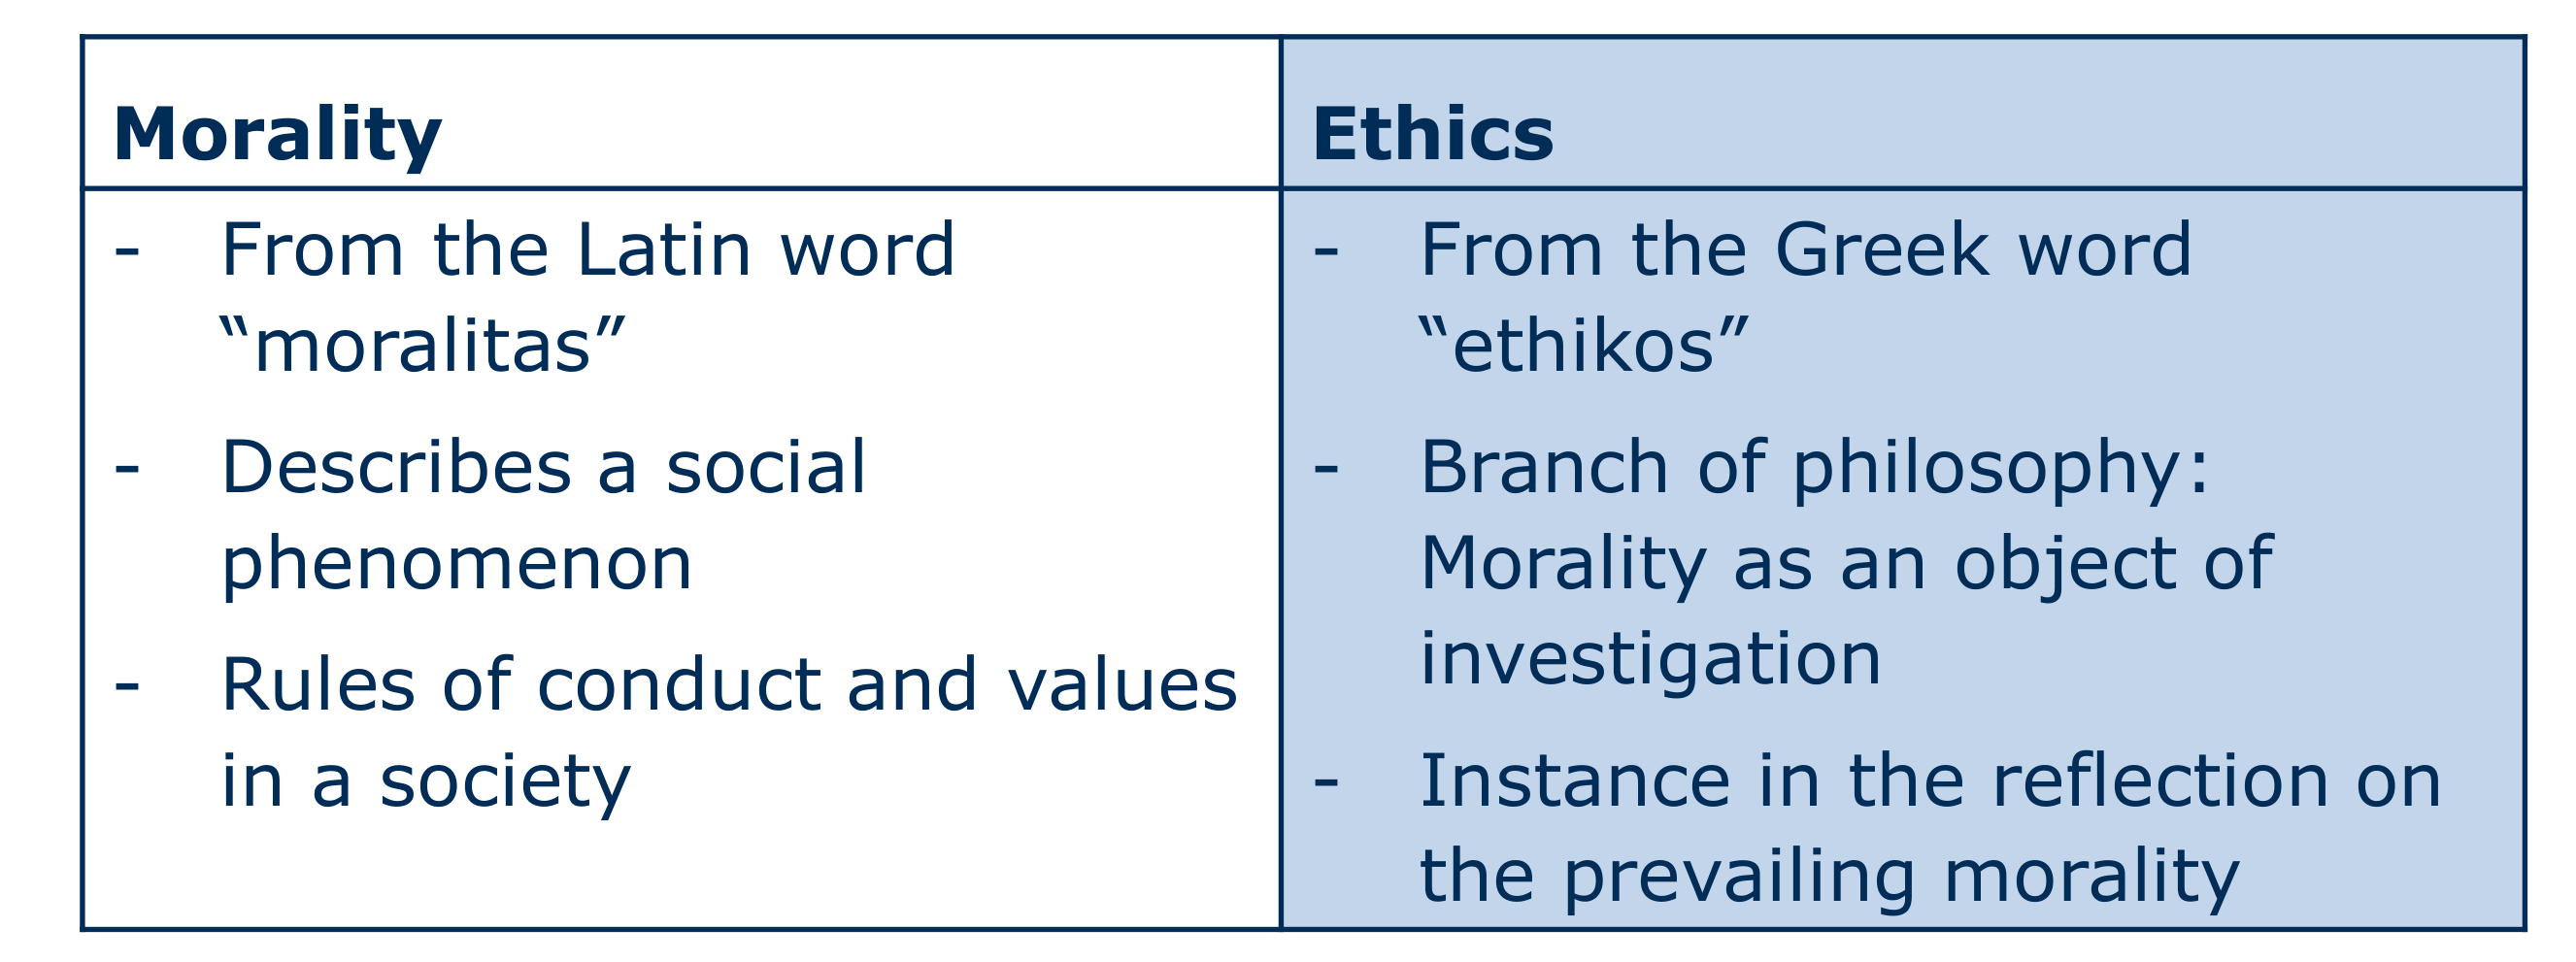
\includegraphics[width=0.6\linewidth]{img/morality_ethics}
	\caption{Comparison between morality and ethics}
	\label{fig:moralityethics}
\end{figure}

\begin{figure}[tbh]
	\centering
	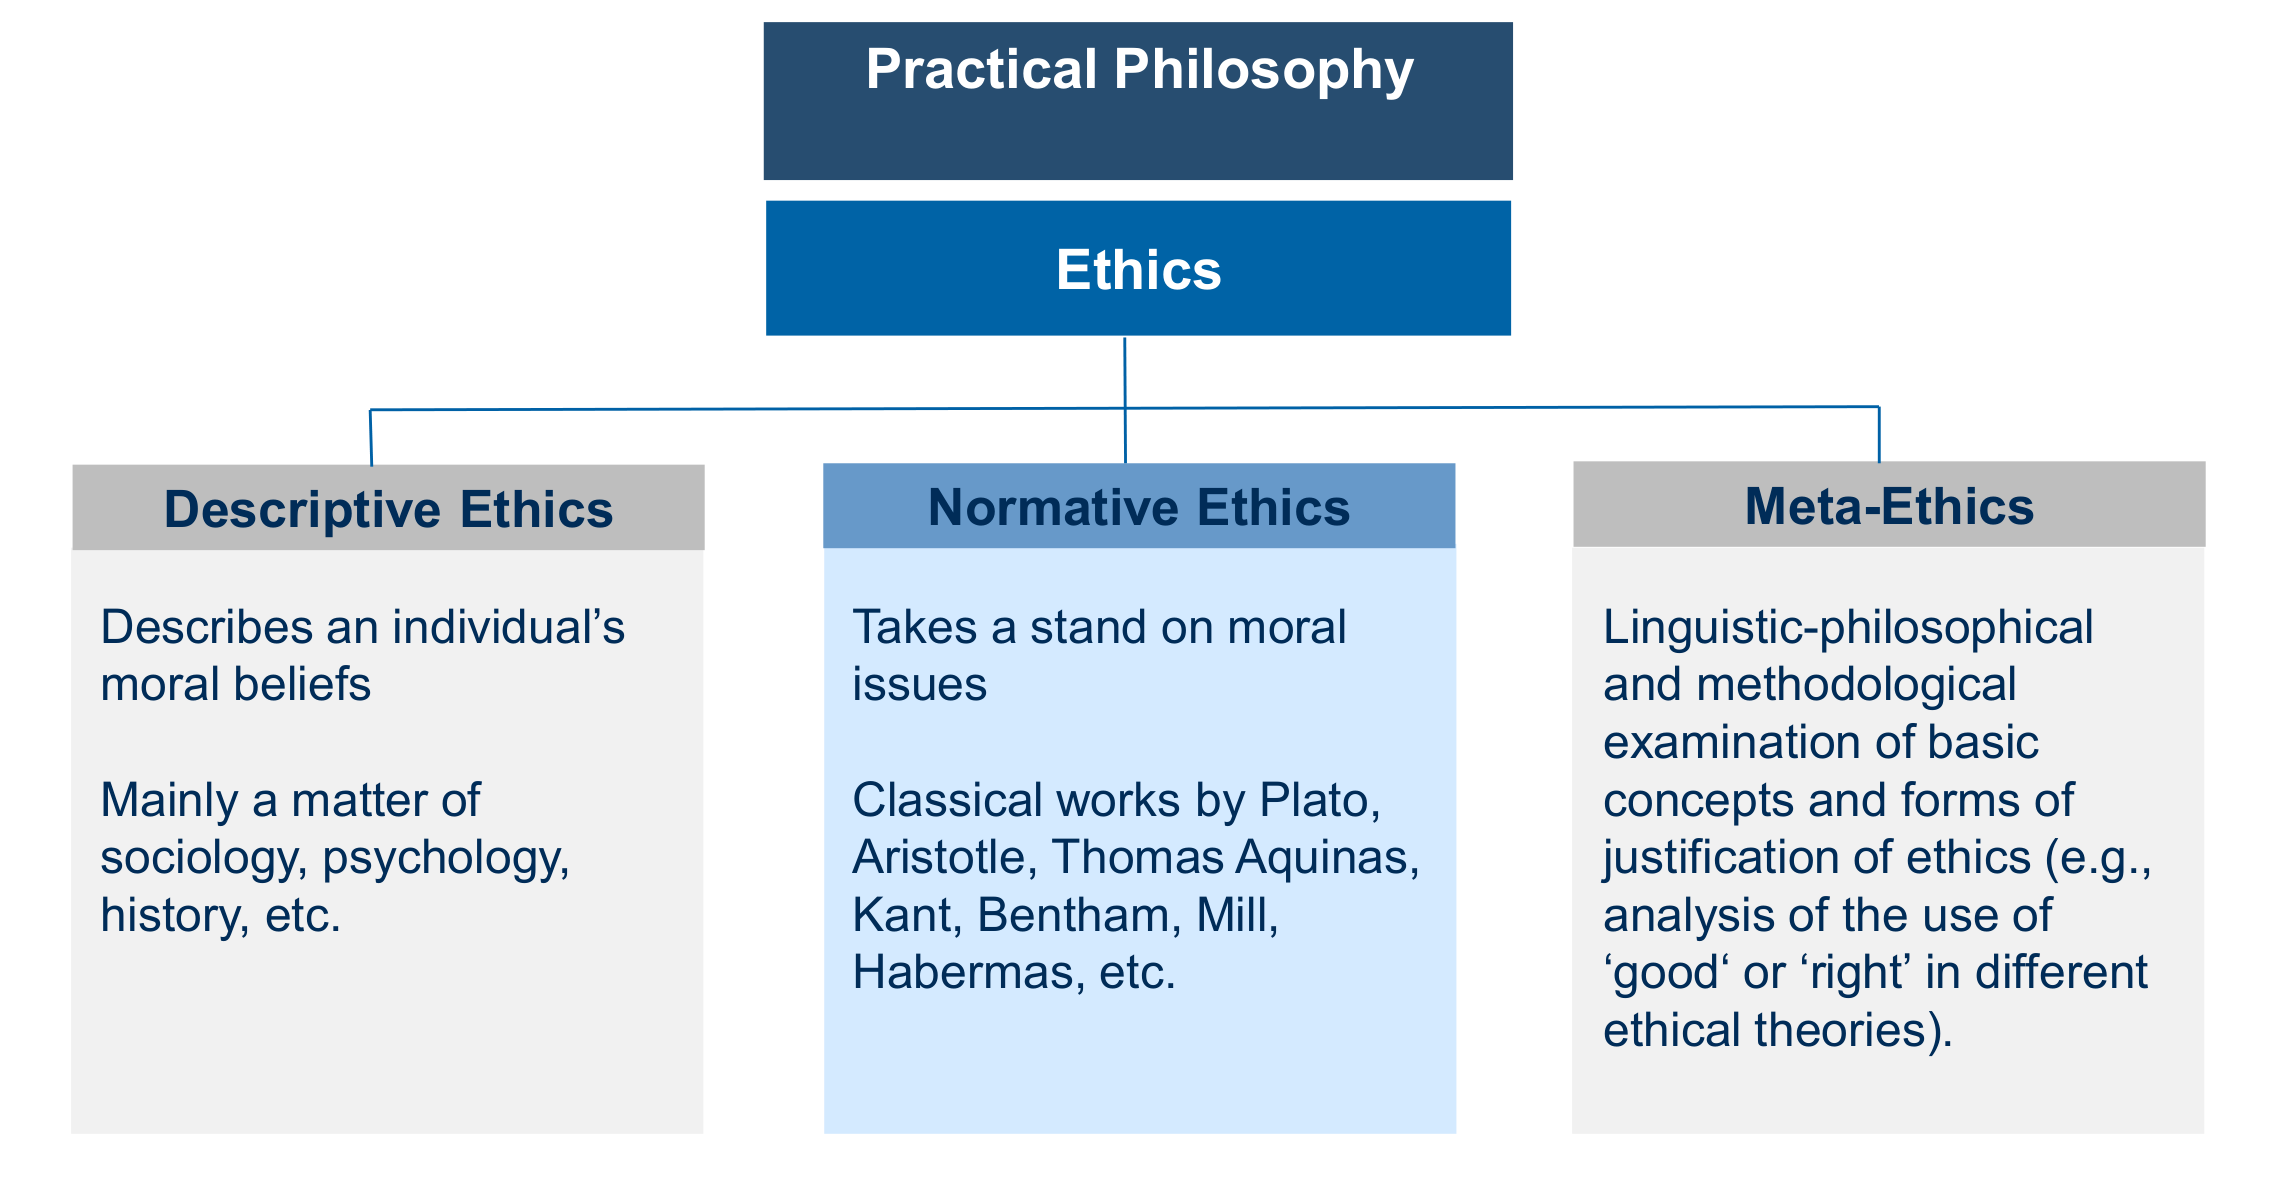
\includegraphics[width=0.8\linewidth]{img/classification_ethics}
	\caption{Classification of ethics}
	\label{fig:classificationethics}
\end{figure}

\begin{figure}[tbh]
	\centering
	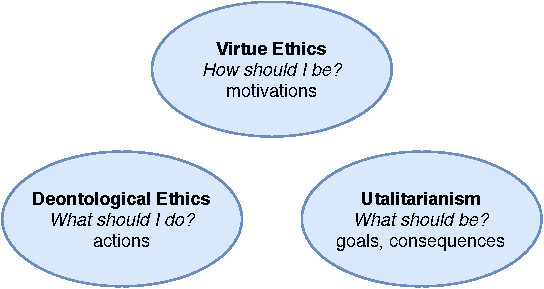
\includegraphics[width=0.8\linewidth]{img/ethics_overview.pdf}
	\caption{Types of ethical arguments discussed in this course}
	\label{fig:overviewethics}
\end{figure}


\section{Virtue Ethics}
Virtue ethics is an ethical mindset that places the emphasis of moral judgment on the motivation for human behaviour. This can either be an isolated thought that prevails at a given moment and causes a particular action to be taken. Or it can be a permanent attitude that develops over time and shapes an individual’s conduct over an entire life \parencite{hubner2018einfuhrung}.

Different virtue ethics focus on the motivation for human action. The actual actions of an individual or the consequences of these actions are not completely disregarded, but are not the prime object of moral judgement. Virtues are often defined in such a way that they strongly recommend an action or desirable consequences. Virtue ethicists do not make any strong recommendations regarding precise actions but are only concerned with the nature of these actions.

The main concepts rooted in ancient Greek philosophy are
\begin{enumerate}
	\item \emph{arête} - excellence or virtue
	\item \emph{phronesis} - practical or moral wisdom
	\item \emph{eudaimonia} - translated as happiness or flourishing
\end{enumerate}

\subsection{Plato's Parts of the Soul and Virtues}
Plato was the first to really think about these aspects and write it down! According to Plato the soul consists of three parts
\begin{itemize}
	\item \textit{Logos}, the part related to reason, which regulates the mind, and is important for insight and judgement
	\item \textit{Thymos}, the part related to anger, strength and assertiveness
	\item \textit{Eros}, the part related to desire, emotions and passion
\end{itemize}

%TODO Check if formatting is still fine
\clearpage
\noindent
He identifies these four cardinal virtues which are true for the individual and the state
\begin{tabularx}{\linewidth}{|l|l|}
	\hline
	\textbf{Virtue} & \textbf{Connection to the Parts of the Soul}\\
	\hline
	Prudence & Reason (rulers) recognizes the appropriate course of action for the soul \\
	Fortitude & Courage (guardians) persists in what has been recognized through reason. \\
	Temperance & All parts of the soul (all citizens) agree that reason (rulers) should rule. \\
	Justice & Every part of the soul contributes (is met if the three other virtues prevail) \\
	\hline
\end{tabularx}

\subsection{Nicomachian Ethics}
Virtue of thinking needs teaching, experience and time, virtue of character (moral virtue) comes about as a consequence of following the right habits. According to Aristotle the potential for this virtue is by nature in humans, but whether virtues come to be present or not is not determined by human nature.

For Aristotle virtues are \textbf{positive}, \textbf{medium character traits} which must be in line with the nature of people, and their actions should be guided by \textbf{reason} and \textbf{insight}.

\begin{definition}
	A \textbf{theological concept} states that if an individual in a community behaves according to the virtue doctrine, he or she will lead a happy life and be considered ethical.
\end{definition}

According to Aristotle the \textbf{highest good} is \textquotedblleft living well\textquotedblright, to always strive for a good life for its own sake. \textbf{Good behaviour is, therefore, the moral goal,} and the highest goal can only be realized in the behaviour itself.

It must be the highest goal of human behaviour to realize reasonableness to the highest degree. Happiness, therefore, consists in acting according to a highly developed reason. This reason is, however, only highly developed if it is of a virtuous nature. Acting out of virtue or virtuous action by the human soul is the highest goal (\textbf{eudaimonia}).

Aristotle distinguishes between two categories of virtue
\begin{tabularx}{\linewidth}{l @{\hskip 2cm} l}
	\textbf{Intellectual} & \textbf{Ethical}\\
	\hline
	Wisdom & Generosity \\
	Prudence & Considerateness \\
	Perception & Courage \\
\end{tabularx}

\subsubsection{Criticism of Aristotelian Ethics}
\begin{itemize}[label=-]
	\item Aristotelian ethics cannot make concrete recommendations
	\item Aristotelian ethics is too relative
	\item The virtuous life does not always lead to a happy life
\end{itemize}

\subsection{Exercise Answers}
\begin{enumerate}
	\item \textbf{What are the three normative approaches introduced in the text?}\\
	\textbf{Virtue ethics}, which emphasises virtues or moral character; \textbf{Deontology}, which emphasises duties or rules; \textbf{Consequentialism}, which emphasises consequences or results. Each approach can consider virtues, consequences, and rules, there is no strict separation in all the cases
	\item \textbf{How is virtue ethics distinguished from the two others?}\\
	Virtue ethics in contrast to an ethical approach focussing on rules (deontology) and the approach focussing on the consequences of actions (consequentialism) focusses on the behaviour or intent of the individual acting virtuous. A virtuous individual is not just so by virtue itself, but has a virtuous mind which lets the person act in a virtuous way in any circumstance, and with ease. Thus such an individual is said to posses "full or perfect virtue" in contrast to a person which has to control his impulses to act virtuous.\\
	What distinguishes virtue ethics from consequentialism or deontology is the \textbf{centrality} of virtue within the theory. Consequentialists will define virtues as traits that yield good consequences and deontologists will define them as traits possessed by those who reliably fulfil their duties, but virtue ethics view them as fundamental. Virtue ethics does not define virtues as traits that yield good consequences or as traits possessed by those who reliably fulfil their duties, but sets the foundation with virtues and vices for other normative notions to be grounded in it.
	\item \textbf{How is arête (excellence or virtue) defined in the text?}\\
	As an excellent trait of character which enables an individual to act in a virtuous manner. To possess a virtue is to be a certain sort of person with a certain complex mindset. A significant aspect of this mindset is the wholehearted acceptance of a distinctive range of considerations as reasons for action.
\end{enumerate}

\section{Deontological Ethics}
Deontological Ethics, \textit{deon} meaning \textquotedblleft obligation\textquotedblright\ in Greek, try to answer the question which norms and actions a person should do to be ethical. The most representative of a deontological approach is by Immanuel Kant:
\begin{itemize}[noitemsep]
	\item The goal of ethics is the observance of what is ethically correct
	\item The ethically good depends on the ethically correct
	\item The ethically correct is \textbf{independent of the consequences}
\end{itemize}

\begin{definition}
	\textbf{Duty} is an action to which a person is obliged. \parencite{kant1870grundlegung}
\end{definition}

\begin{definition}
	\textbf{The Categorical Imperative} is to act as if the maxims of your behaviour could, through your will, serve at any time as the basis of a general law. \parencite{kant1870grundlegung}
\end{definition}

\begin{definition}
	\textbf{Morality} is to do what is your duty (to follow absolutely valid norms of action) and do it out of duty (with a moral attitude).
\end{definition}

\subsection{Kant's Deontological Ethics}
Kant's deontological ethics are based on the idea that only free will that rules an autonomous action determines the ethical quality of an action, and that every individual has dignity and a free will. As a result, only the responsibility for actions resulting from freedom to act or autonomy can be judged ethically.

Kant's conception of freedom is to act freely, that is to act autonomously and guided by a law given by the individual itself. The opposite of autonomy is heteronomy, that is to act according to desires the individual has not chosen itself. While the value of an action can only be measured by the intention behind it, the quality of this intention can only be judged by the \textbf{action maxim} chosen by the subject. This capacity to act freely is what gives human lives its special dignity, and to respect this dignity means regarding people not just as a means to an end but as ends in themselves.

\subsection{The Categorical Imperative}
An action is morally correct if it follows maxims which are good in themselves.
\begin{enumerate}
	\item Act only according to a maxim according which you can also want it to become a universal law
	\item Act as if the maxims of your behaviour could, through your will, serve at any time as the basis of a universal law of nature
	\item Act as if you always need humanity, both in yourself and in the person of everyone else, as an end in itself, never merely as a means to an end
\end{enumerate}

\subsection{Human Rights}
Human rights are basic rights and every human being is entitled to them by nature. These rights apply \textbf{regardless of place and time} and are codified in the United Nations Universal Declaration of Human Rights (1948).

\subsection{Principles of Discourse Ethics}
\begin{itemize}
	\item Communicative action as a referential framework for the lifeworld of a society
	\item Solving conflicts by means \textbf{non-violent communication} and with \textbf{rational arguments}
	\item \textbf{Human rights} as basis
	\item In an ideal, practical discourse all those involved participate and agree to a norm in the end
	\item Reasons must be given, Fairness and Consequences
\end{itemize}

\begin{figure}[tbh]
	\centering
	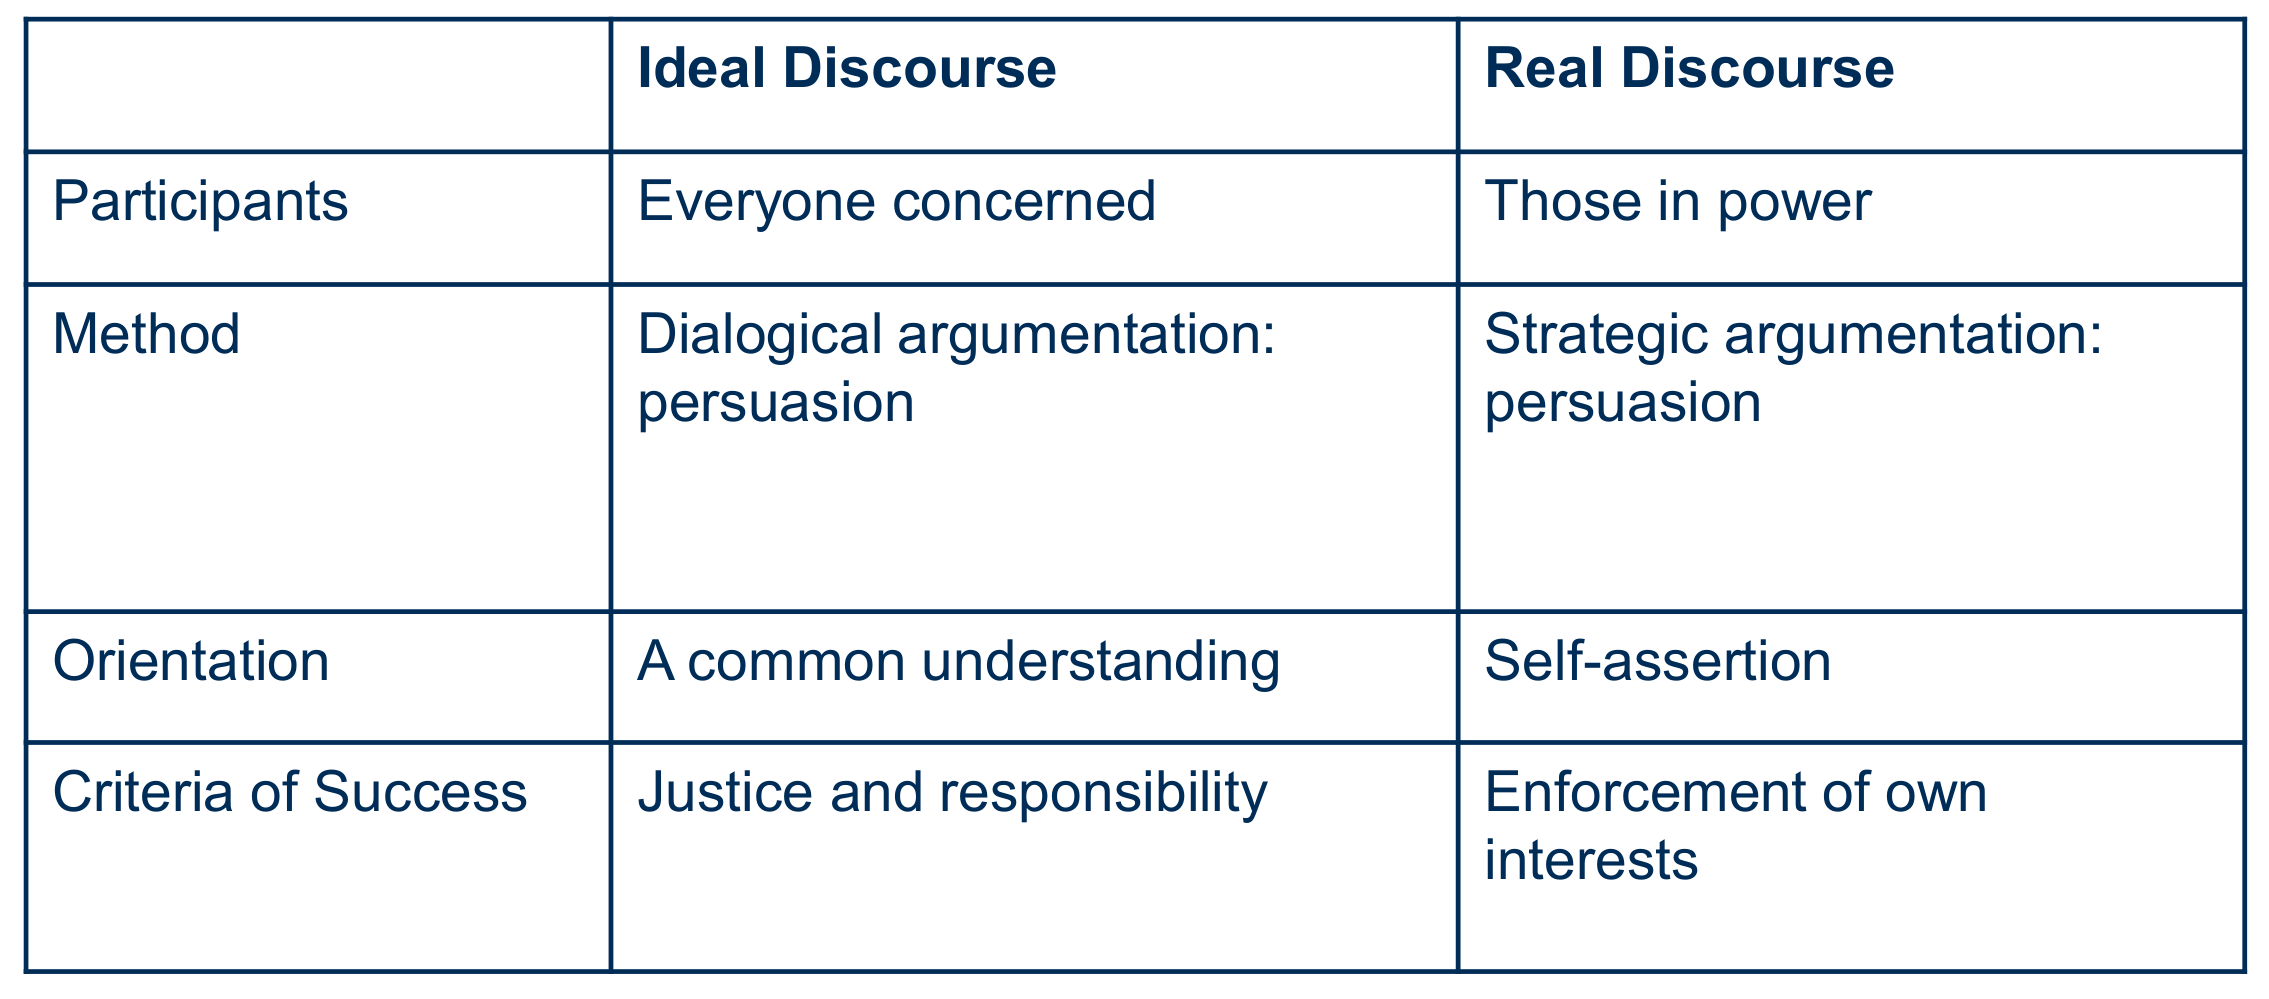
\includegraphics[width=0.8\linewidth]{img/discourse_comparison}
	\caption{Comparison between an ideal discourse and how real discourses often take place}
	\label{fig:discoursecomparison}
\end{figure}

%TODO Check if formatting is still fine
\clearpage

\subsection{A Theory of Justice}
The original position is the contract-theoretical justification of principles. Justice should be fairness, and there is a principle of impartiality or a "veil of ignorance".

\vspace{1em}
\noindent
\textbf{Concepts}
\begin{itemize}
	\item \textbf{Distributive justice}, to each the same, according to the performance, according to the needs
	\item \textbf{Retributive justice}, exchange of equivalent values, according to the work performed, practical or market value
	\item \textbf{Corrective justice}, reparation, compensation, sanctions
	\item \textbf{Procedural justice}
	\begin{itemize}
		\item perfect, one distributes the other chooses
		\item imperfect, court trials or political decisions
		\item pure, a draw, randomness
	\end{itemize}
\end{itemize}
\vspace{1em}
\noindent
\textbf{Principles}
\begin{enumerate}
	\item Each person has the same indefeasible claim to a fully adequate scheme of equal basic liberties, which scheme is compatible with the same scheme of liberties for all;
	\item Social and economic inequalities are to satisfy two conditions:
	\begin{enumerate}
		\item They are to be attached to offices and positions open to all under conditions of fair equality of opportunity;
		\item They are to be to the greatest benefit of the least-advantaged members of society (the difference principle; according to the MaxMin principle in game theory)
	\end{enumerate}
\end{enumerate}

\subsection{Exercise Answers}
\begin{enumerate}
	\item What are weaknesses of the deontological approach?\\
	Deontology holds that some choices cannot be justified by their effects and thus are morally always forbidden. But this leads to justification for helping in unjust acts and still be morally clean. For example driving a robber to his robbery target. It also allows that each one of us is morally sound, but the world is becoming much worse. Also, in my opinion the sole focus on the moral self is unattractive and per definition selfish.
\end{enumerate}

%TODO Check if formatting is still fine
\clearpage
\section{Utilitarian Ethics}
The term utilitarianism is a form of consequentialism and encompasses theoretical approaches of ethics which evaluate the moral value of an action based on its consequences.
\begin{definition}
	\textbf{Utilitarianism}, the ethics of maximising utility, makes the moral evaluation of an action or a rule of action dependent on its consequences. Being moral is to achieve maximum utility (happiness or well-being) for the highest number of people.
\end{definition}
Happiness is understood as a net balance of positive and negative states of well-being.  An action is good if it increases both individual happiness and the happiness of the community.

\vspace{1em}
\noindent
\textbf{Basic Principles}
\begin{enumerate}
	\item Consequentialism\\
	Assessing the consequences of an action, evaluating the common wellbeing
	\item Eudemonism\\
	Happiness or wellbeing as the most important good
	\item Teleological Ethics\\
	The goal is maximizing happiness in the world
	\item Individualism\\
	Effects, aggregated to each individual; Individual happiness is added, individual suffering deducted
	\item Universalism\\
	Individuals have the same weighting (maybe even animals)
\end{enumerate}

\begin{figure}[tbh]
	\centering
	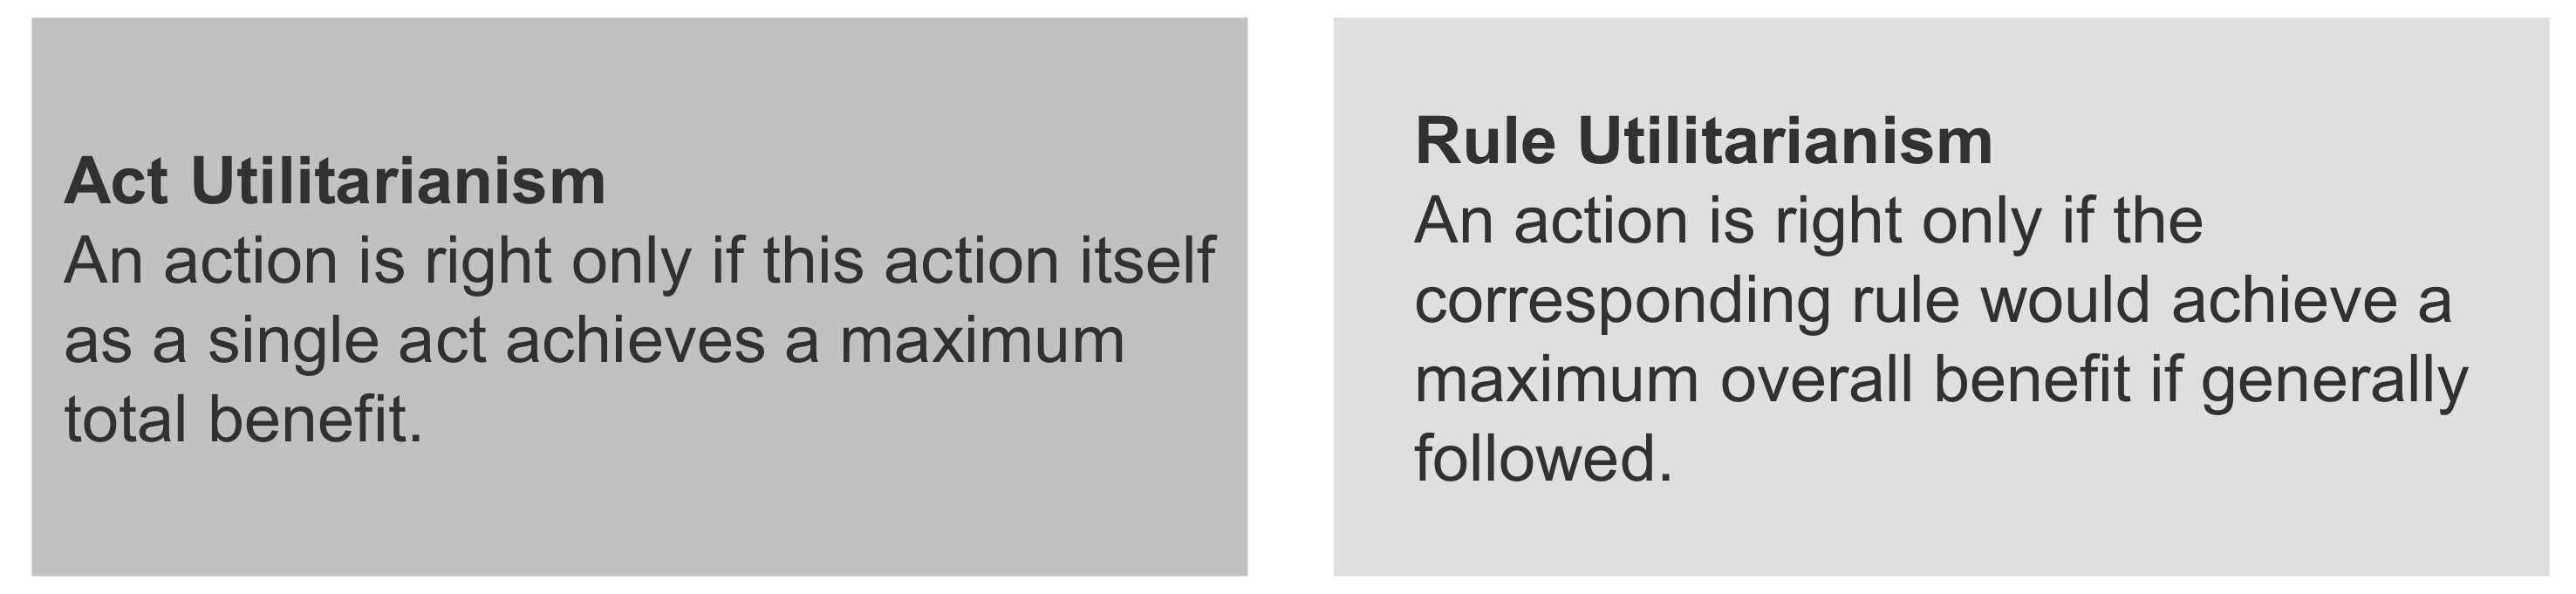
\includegraphics[width=0.8\linewidth]{img/act-rule-utilitarianism}
	\caption{Option: Decisive decision-making criterion are action or rule}
	\label{fig:act-rule-utilitarianism}
\end{figure}

\begin{figure}[tbh]
	\centering
	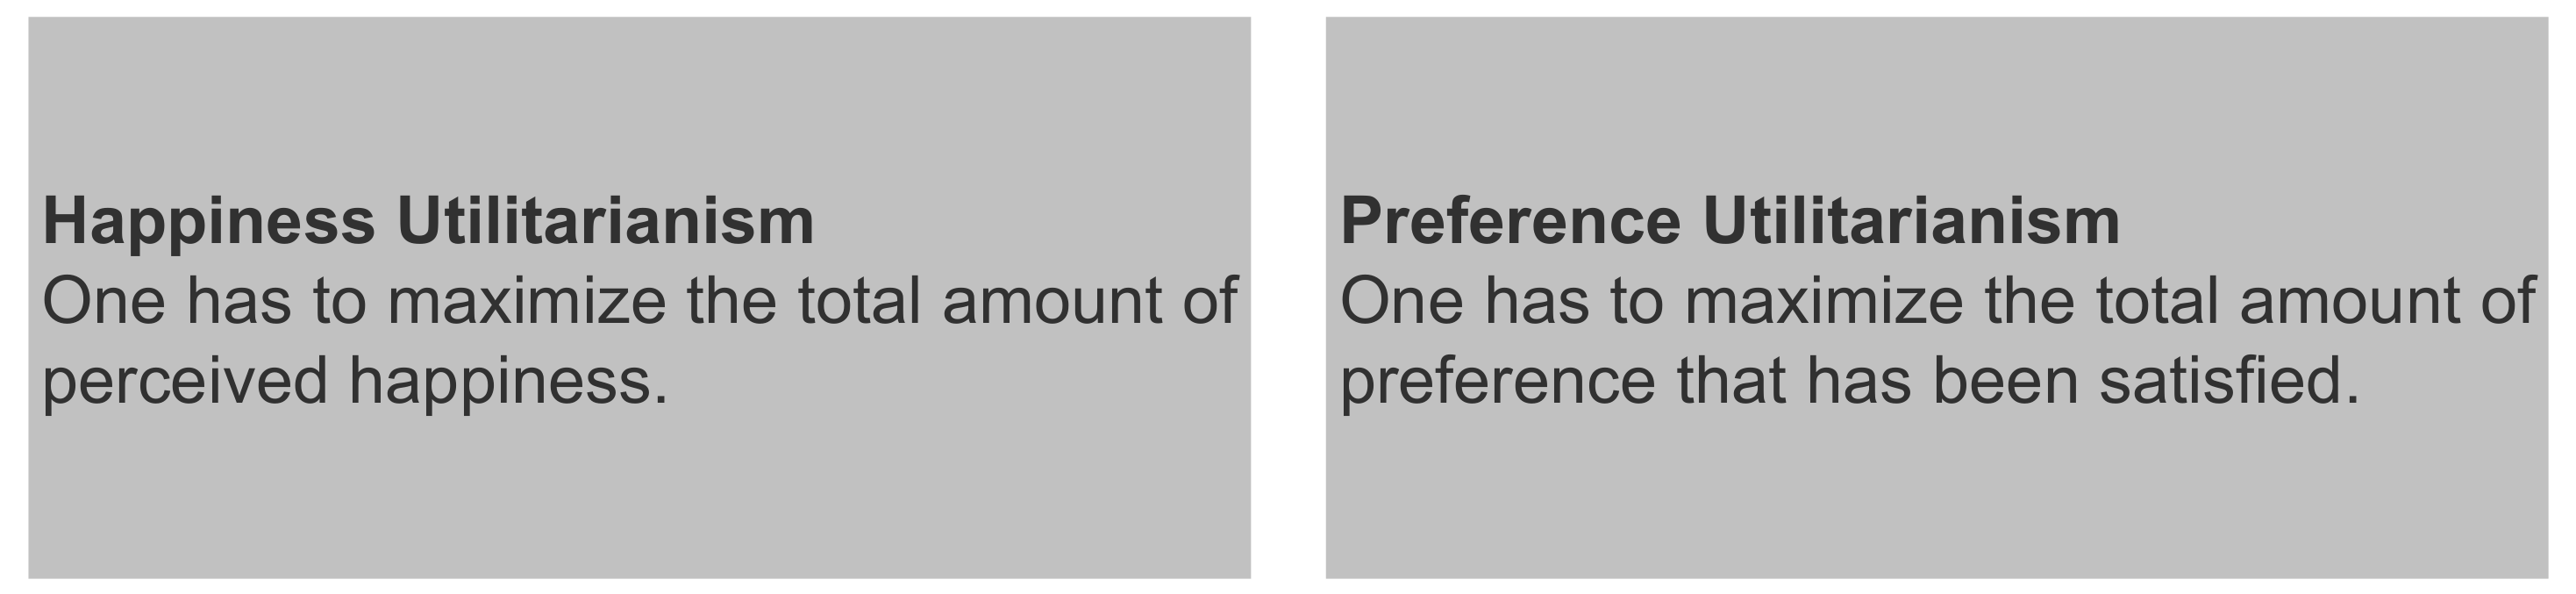
\includegraphics[width=0.8\linewidth]{img/happiness-preference-utilitarianism}
	\caption{Option: happiness or preference}
	\label{fig:happiness-preference-utilitarianism}
\end{figure}

According to Jeremy Betham (1748-1832) the core thesis is the \textit{Maximum Happiness Principle}, the striving for pleasure and avoidance of suffering. He introduces the \textbf{utility principle} which appraises every action according to the extent to which it increases the happiness of the community more than it diminishes it.

%TODO Check if formatting is still fine
\clearpage
Bentham postulates the \textbf{felicific calculus} (also called utility or hedonistic calculus) to calculate the degree or amount of pleasure that a specific action is likely to cause, in principle this allows to determine the moral status of any action.
\begin{enumerate}[nosep]
	\item \textbf{Intensity}\\
	How strong is the pleasure?
	\item \textbf{Duration}\\
	How long will the pleasure last?
	\item \textbf{Certainty or uncertainty}\\
	How likely or unlikely is it that the pleasure will occur?
	\item \textbf{Propinquity or remoteness}\\
	How soon will the pleasure occur?
	\item \textbf{Fecundity}\\
	The probability that the action will be followed by sensations of the same kind.
	\item \textbf{Purity}\\
	The probability that it will not be followed by sensations of the opposite kind.
	\item \textbf{Extent}\\
	How many people will be affected?
\end{enumerate}

\section{Applied Ethics and Sustainable Development}
The current world is an amalgamation of world views and different symbolic organisation with differing actions and options (\textbf{pluralism}). There is a complexity of contexts and situations with conflicts of interests, orientation problems and possible conflicts of conscience. Ethics can be a basis for reasoned judgements and actions which can help shape and design of just institutions.

\begin{definition}
	\textbf{Applied ethics} is a philosophical discipline of problem-related ethics with moral problems in selected areas. Discourses and catalogues of standards on single topics with a focus on a specific theme.
\end{definition}

\begin{figure}[tbh]
	\centering
	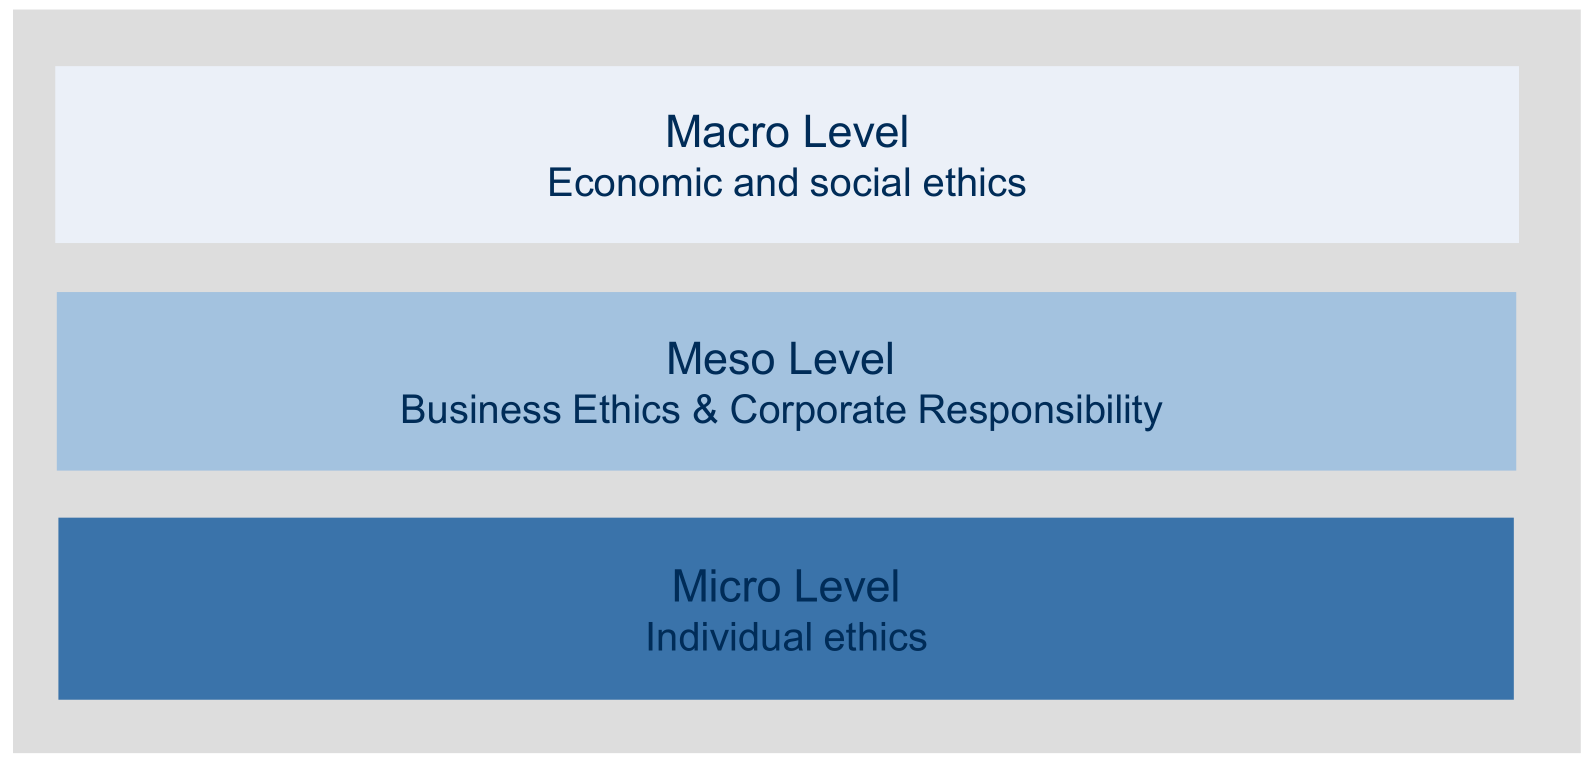
\includegraphics[width=0.6\linewidth]{img/applied_ethics_level}
	\caption{Levels of applied ethics}
	\label{fig:appliedethicslevel}
\end{figure}

\begin{itemize}
	\item Macro Level\\Economics and social ethics; the state decides laws, framework conditions and guiding principles
	\item Meso Level\\Business Ethics and Corporate Responsibility; a company decides on its working conditions, product range, handling of its resources, and on the corporate philosophy and culture
	\item Micro Level\\Individual Ethics; the individual decides on its behaviour
\end{itemize}

\subsubsection{Relativism Debate}
Relativism denies the universal validity of ethical standards. Relativism principle states that there is no rational method for testing ethical principles. But as a counterargument one can observe that there is an independent standpoint of morality with rational evaluation of principles, values and justifications.

\subsection{Sustainable Development}
\begin{definition}
	Sustainable development is development that meets the needs of the present without compromising the ability of future generations to meet their own needs.
\end{definition}
The model of sustainability has the ethical starting point of having the responsibility for future generations and thus the postulate of intergenerational justice.
\begin{definition}
	Responsibility is the state or fact of having a duty to deal with something or of having control over someone.
\end{definition}
It means the obligation to act as a subject for an object. \parencite{gobel2013unternehmensethik}

\begin{figure}[tbh]
	\centering
	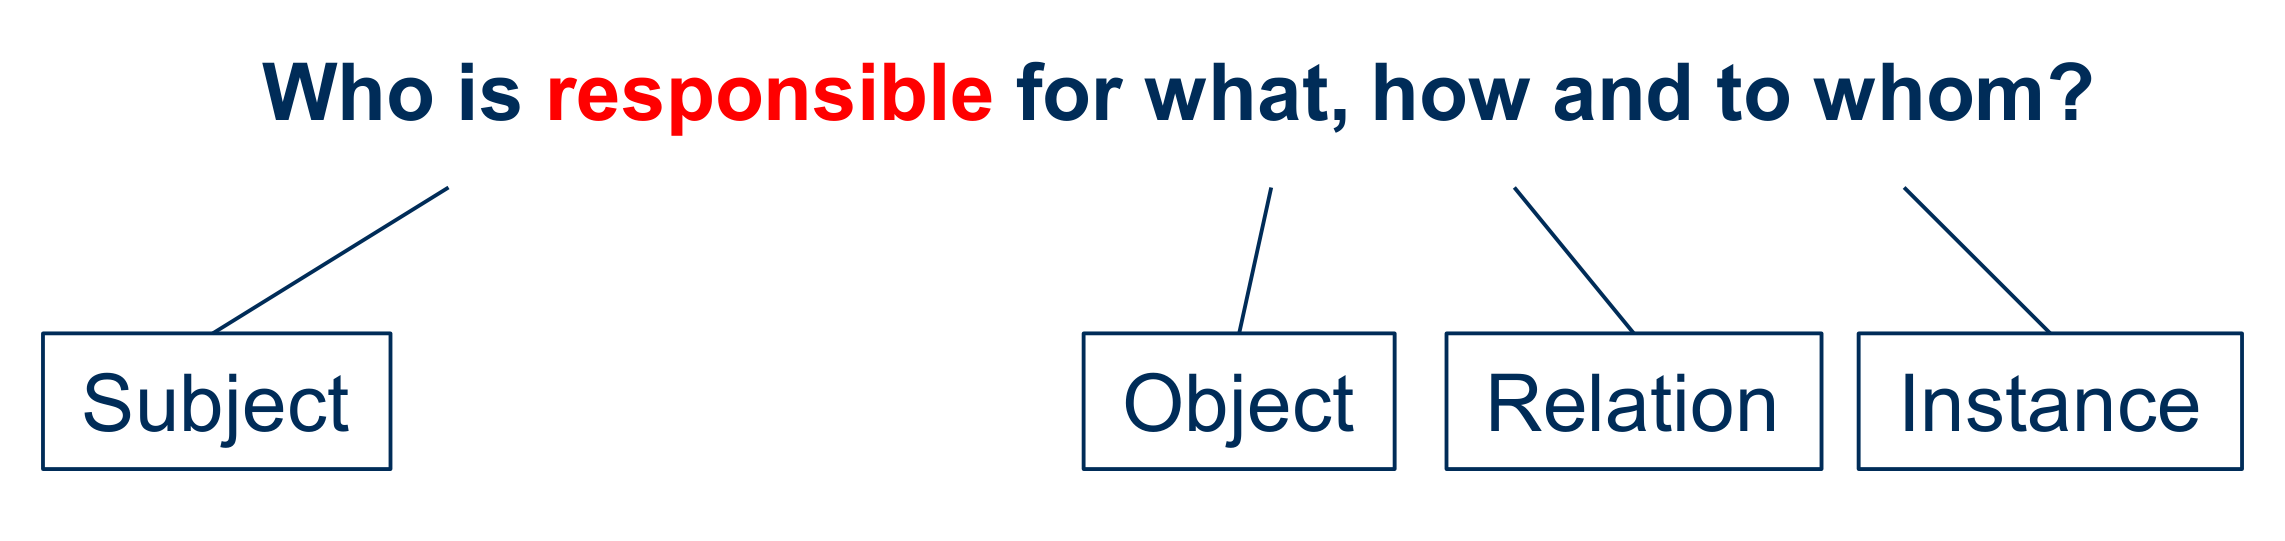
\includegraphics[width=0.6\linewidth]{img/responsibility}
	\caption{Elements of responsibility}
	\label{fig:responsibility}
\end{figure}

\subsubsection{Responsibility - Level I (Anthropocentric)}
\begin{enumerate}
	\item Everyone only takes care of himself
	\item In addition to themselves, everyone takes care of their family, friends and acquaintances as well as their immediate ancestors
	\item Everyone takes care of himself, those close to him and his fellow citizens or the people to whom he belongs, including the immediate heritage of the past
	\item Everyone takes care of himself, those close to him, his own people, and the present living generations of all humanity
	\item Everyone takes into consideration himself, those who are close to him, his own people, the present living generations of all humanity, all ancestors and those born after, that is, humanity as a whole
\end{enumerate}

\subsubsection{Responsibility - Level II (Physiocentric)}
\begin{enumerate}
	\item Everybody takes \textbf{humanity as a whole} and \textbf{all consciously feeling living beings} (individuals and species) into consideration
	\item Everyone takes \textbf{all living things} (individuals and species) into consideration
	\item Everyone shows consideration \textbf{for everything}
\end{enumerate}

%TODO Check if formatting is still fine
\clearpage
\subsubsection{Sustainability Models}
\begin{tabularx}{\linewidth}{|X|X|}
	\hline
	\textbf{Weak Sustainability} & \textbf{Strong Sustainability}\\
	\hline
	Maintain or increase aggregated natural, social and economic capital. & Keeping or increasing natural capital constant \\
	\hline
	Loss of natural capital can be compensated by social and economic capital. & Loss of natural capital is an injustice to future generations \\
	\hline
	Measuring method: real savings & Measurement method: Global Footprint \\
	\hline
	Benefit principle & Precautionary principle \\
	\hline
\end{tabularx}

\subsubsection{United Nations 2030 Agenda}
\begin{figure}[H]
	\centering
	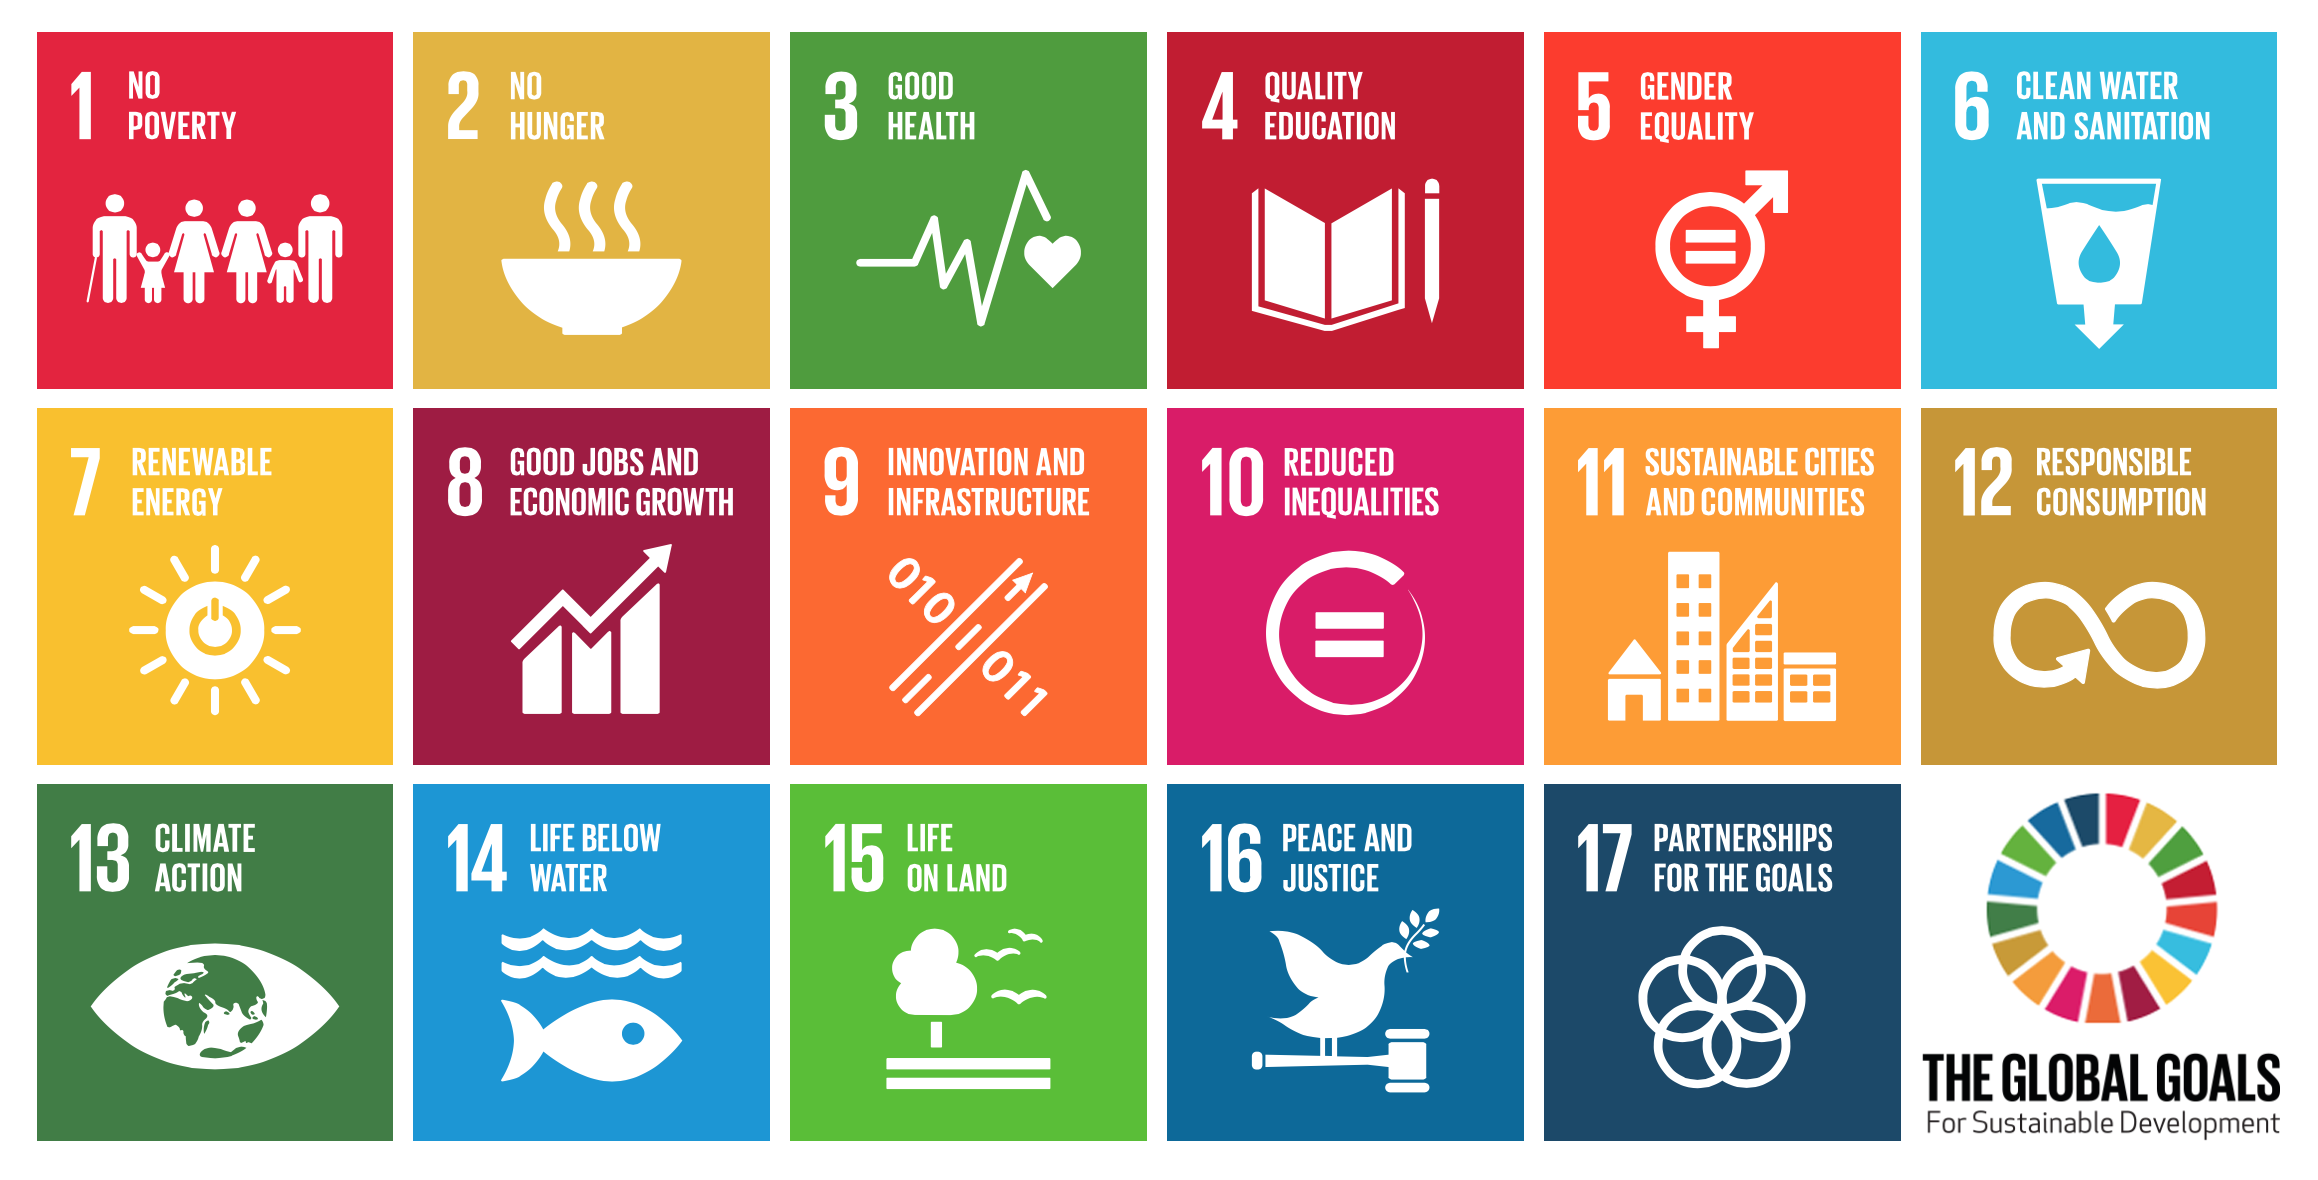
\includegraphics[width=0.9\linewidth]{img/sustainable_development_goals}
	\caption{United Nations Sustainable Development Goals}
	\label{fig:sustainabledevelopmentgoals}
\end{figure}

\subsection{Key Challenges}
\begin{itemize}
	\item Instability
	\item Implementation\\The laws have to be implemented on a local level, this process is slow and decentralised
	\item Governance\\Politicians are not that interested in implementing changes, as they have very short term goals (next election)
\end{itemize}

\section{Future and Digital Ethics}
Future ethics concerns itself with the responsibility of actions with regard to consequences, especially the impact they have on future generations, and thus deals with issues that have long-term effects on people, society and nature, and which are thus not easily foreseeable.

Hans Jonas was a philosopher whose research into Gnosticism was the foundation work for a long time. Furthermore, he wrote the book \textit{The Imperative Of Responsibility} which centres on social and ethical problems created by technology and its use. His ideas encompassed that nature has intrinsic value, and that humanity has the duty to care for the future of all nature on this planet as a necessary condition of it's own \parencite{jonas1984imperative}. Complications are the limited predictions one can make based on current knowledge and the increasing vulnerability of nature. He argues that humanity should veer from the idea of a better life in terms of greater consumption towards a better life of ethical and cultural quality and of sociopolitical order.

\subsection{Ecological Imperative}
\begin{itemize}[label=-]
	\item Act so that the effects of your actions are compatible with the permanence of real human life on earth.
	\item Act so that the effects of your actions are not destructive to the future possibility of such life.
	\item Do not endanger the conditions for the indefinite existence of mankind on earth.
	\item Include in your present choice the future integrity of man as a co-object of your will.
\end{itemize}

\subsection{Scheme for Ethical Decision Making}
\begin{enumerate}
	\item Analyze facts\\
	Collect basic information and scientific findings
	\item Analyze interests and areas of conflict\\
	Identify stakeholders with their interests, claims and rights at a micro, meso and macro level
	\item Evaluate and justify\\
	Evaluation and consideration, that is virtue ethics, deontological and teleological ethics; statement and justification
	\item Propose measures\\
	Measures for implementation on a micro, meso and macro level
\end{enumerate}

\subsection{Information and Digital Ethics}
\begin{definition}
	\textbf{Information ethics} is a field of applied ethics that deals with the handling of information and information and communication technologies under moral and ethical aspects.
\end{definition}

The motivation of information ethics lies in the growing importance of information, which is also described as a change towards an information society. When dealing with knowledge and information in virtual spaces, new moral concepts and norms emerge (for example hacker ethics, netiquette), which are investigated and discussed in the context of information ethics.

\begin{definition}
	\textbf{Digital ethics} is a subcategory of information ethics and partly a continuation of approaches of media ethics. It examines how digital media and technologies are used by individuals and organisations, the social context they are used in, and which approaches can be negotiated to solve problems and conflicts that arise in this context.
\end{definition}

\subsubsection{Areas of Application}
\begin{itemize}
	\item Proprietary rights to information
	\item Aspects of freedom of information
	\item Overcoming a digital divide between people with and without access to information
	\item Informational self-determination and the protection of privacy in view of growing possibilities of surveillance (data privacy)
	\item Necessity of restrictions on the dissemination of information due to the protection of personality and/or child protection
	\item Economization and the digital transformation of the work environment
	\item Privacy and data protection
	\item Change in values in the course of digitization, especially values such as privacy and autonomy
	\item Cyberbullying
	\item Doxxing or Hacking
	\item Artificial intelligence and the increasing importance of robotics
	\item Points of contact with machine ethics
	\item Human-technology interaction
\end{itemize}

\subsubsection{Central Questions}
\begin{itemize}
	\item Opportunities and side effects of technology
	\item Risks of technology
	\item Influence of technology on the human self-image and the culture we want to live in
\end{itemize}

\subsection{Conflicting Goals}
\textbf{Balancing values}
\begin{itemize}[label=-]
	\item Accessibility versus Privacy
	\item Individualisation and Personalisation versus Privacy
	\item Customer satisfaction versus Freedom of choice
\end{itemize}
\textbf{Balancing interests}
\begin{itemize}[label=-]
	\item Insight versus Privacy
	\item Law enforcement versus Privacy
\end{itemize}
\textbf{Impact assessment}
\begin{itemize}[label=-]
	\item Future options versus appropriate data use
\end{itemize}

\subsection{Exercise}
Sustainable information systems can carry the values of the engineers and designers. This can help in recognising potential customer value propositions and customer needs. However, sustainability is in itself a value which depends on a holistic long-term value consideration, and is thus not likely to be considered by managers and companies with short-term profit orientations.

%TODO Check if formatting is still fine
\clearpage
\section{Business Ethics and Code of Ethics}
Subject areas of Business Ethics:
\begin{itemize}
	\item Corporate Ethics
	\item Consumer Ethics
	\item Economic Order
	\item Financial Market Ethics
\end{itemize}
\begin{definition}
	Business ethics is a field of applied ethics. It does not offer applicable knowledge (how to do something) but critical \textbf{normative orientation knowledge} (what to do).
\end{definition}

\subsection{Business Ethics Approaches Overview}
\subsubsection{Republican Approach}
The profit principle of the market is sacrosanct and not questioned, so employing ethics always costs money. Standards guiding action should be developed in dialogue and consensus oriented in the way that the better argument has priority. Ethical leadership contributes to the legitimisation of corporate action.

The shortcomings of this approach are that ideal discourse is difficult to have and that the profit principle is not critically investigated.

\subsubsection{Economic Approach}
The economic liberal approach strives for an economic justification of ethics. The market economy is not questioned, as it leads to the most welfare in society. The place of morality is in the general regulatory framework. Deficits arise when the regulatory framework reacts with a time lag to technical, economic, and social changes.

The shortcomings lie in that the idea of a regulatory framework order is too idealistic, and not applicable to the globalised world (no global regulatory institution). It focusses more on rule-conformal behaviour and not on moral consciousness.

\subsubsection{Integrative Approach}
The entrepreneurial pursuit of success and profit is subordinated to the normative condition of legitimacy. The purpose of all entrepreneurial activity is the creation of value to satisfy individual human and social needs. Ethics is thus a task for the entire company including measures to promote corporate responsibility.

The shortcomings of this approach are that it presupposes a basic conflict between ethics and business, it does not try to solve the conflict but instead postulates the ethics as centre stage.

\subsection{Recognising an Ethical Issue}
Leading questions are:
\begin{itemize}
	\item Is this issue about more than what is legal or what is most efficient? If so, in what way?
	\item Does this decision involve a choice between a good and bad alternative, or perhaps between two "goods" or two "bads?"
	\item Could this decision or situation be damaging to an individual or a group?
\end{itemize}

\subsection{Codes of Conduct}
The codes of conduct (CoC) are a compliance instrument for ethics management in companies, sectors or industries. They describe or establish compliance with certain standards and rules of conduct, and are part of the risk management. They provide a value framework within which a company or industry wishes to conduct its business.

Often at least these three areas are covered
\begin{itemize}
	\item Business ethics\\
	bribery, competition, conflicts of interest, legal provisions
	\item Responsibility for the environment
	\item Social responsibility\\
	human rights, employees, unions
\end{itemize}

\section{Corporate Responsibility}
Traditional Definitions of Corporate Responsibility
\begin{definition}
	Corporate Social Responsibility is the ongoing commitment of companies to contribute to economic development while improving the quality of life of employees, their families, the community and society as a whole.
\end{definition}

\begin{definition}
	$[...]$ socially responsible companies try to maximize profits while improving the welfare of other stakeholders.
\end{definition}

\vspace*{1em}
\noindent
Definition that would be signed by most economists
\begin{definition}
	Corporate responsibility describes the way a company takes responsibility for the solution of societal challenges while pursuing the company’s overriding objective.
	\begin{itemize}
		\item corporate: relating to a company or corporation
		\item responsibility: something for which one is responsible; a duty, an obligation, or a burden
	\end{itemize}
\end{definition}

\subsection{Categories of Corporate Responsibility Topics}
\begin{itemize}
	\item Responsibility or Accountability
	\item Human Rights
	\item Working Conditions
	\item Ethical behavior
	\item Corporate Governance
	\item Environmental Protection and Conservation
	\item Market and Consumption
\end{itemize}

\subsection{Impact on Supply Chain}

\begin{figure}[H]
	\centering
	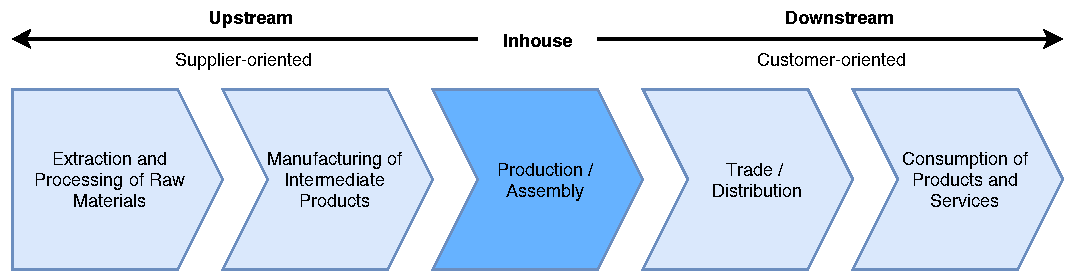
\includegraphics[width=0.85\linewidth]{img/corporate_responsibility_stages.pdf}
	\caption{Corporate responsibility topics may arise in different locations in the supply chain, for example working conditions in mines (upstream), sexual harassment inside the main office (inhouse), or perpetuation of racism or sexism in trading (downstream)}
\end{figure}

\begin{figure}[htb]
	\centering
	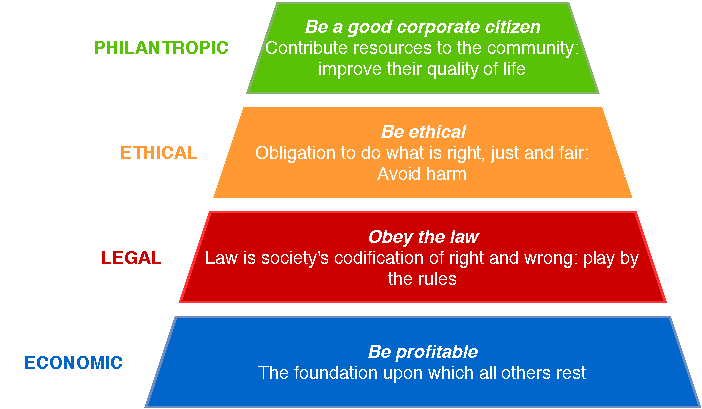
\includegraphics[width=0.7\linewidth]{img/caroll_pyramid_corporate_responsibility.pdf}
	\caption{The CSR pyramid intends to portray the distinct components which, taken together, constitute the whole of CSR \parencite{caroll1991pyramid}}
\end{figure}

\begin{figure}[htb]
	\centering
	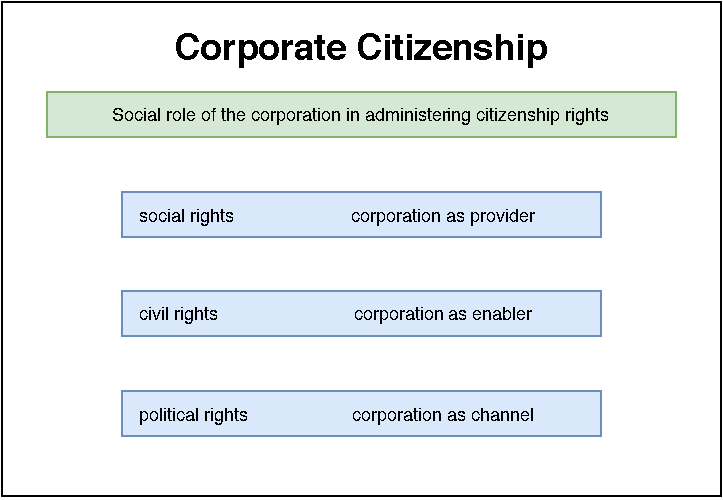
\includegraphics[width=0.7\linewidth]{img/Matten_Crane_corporate_citizenship.pdf}
	\caption{The Matten and Crane Model of corporate citizenship}
\end{figure}

\begin{figure}[htb]
	\centering
	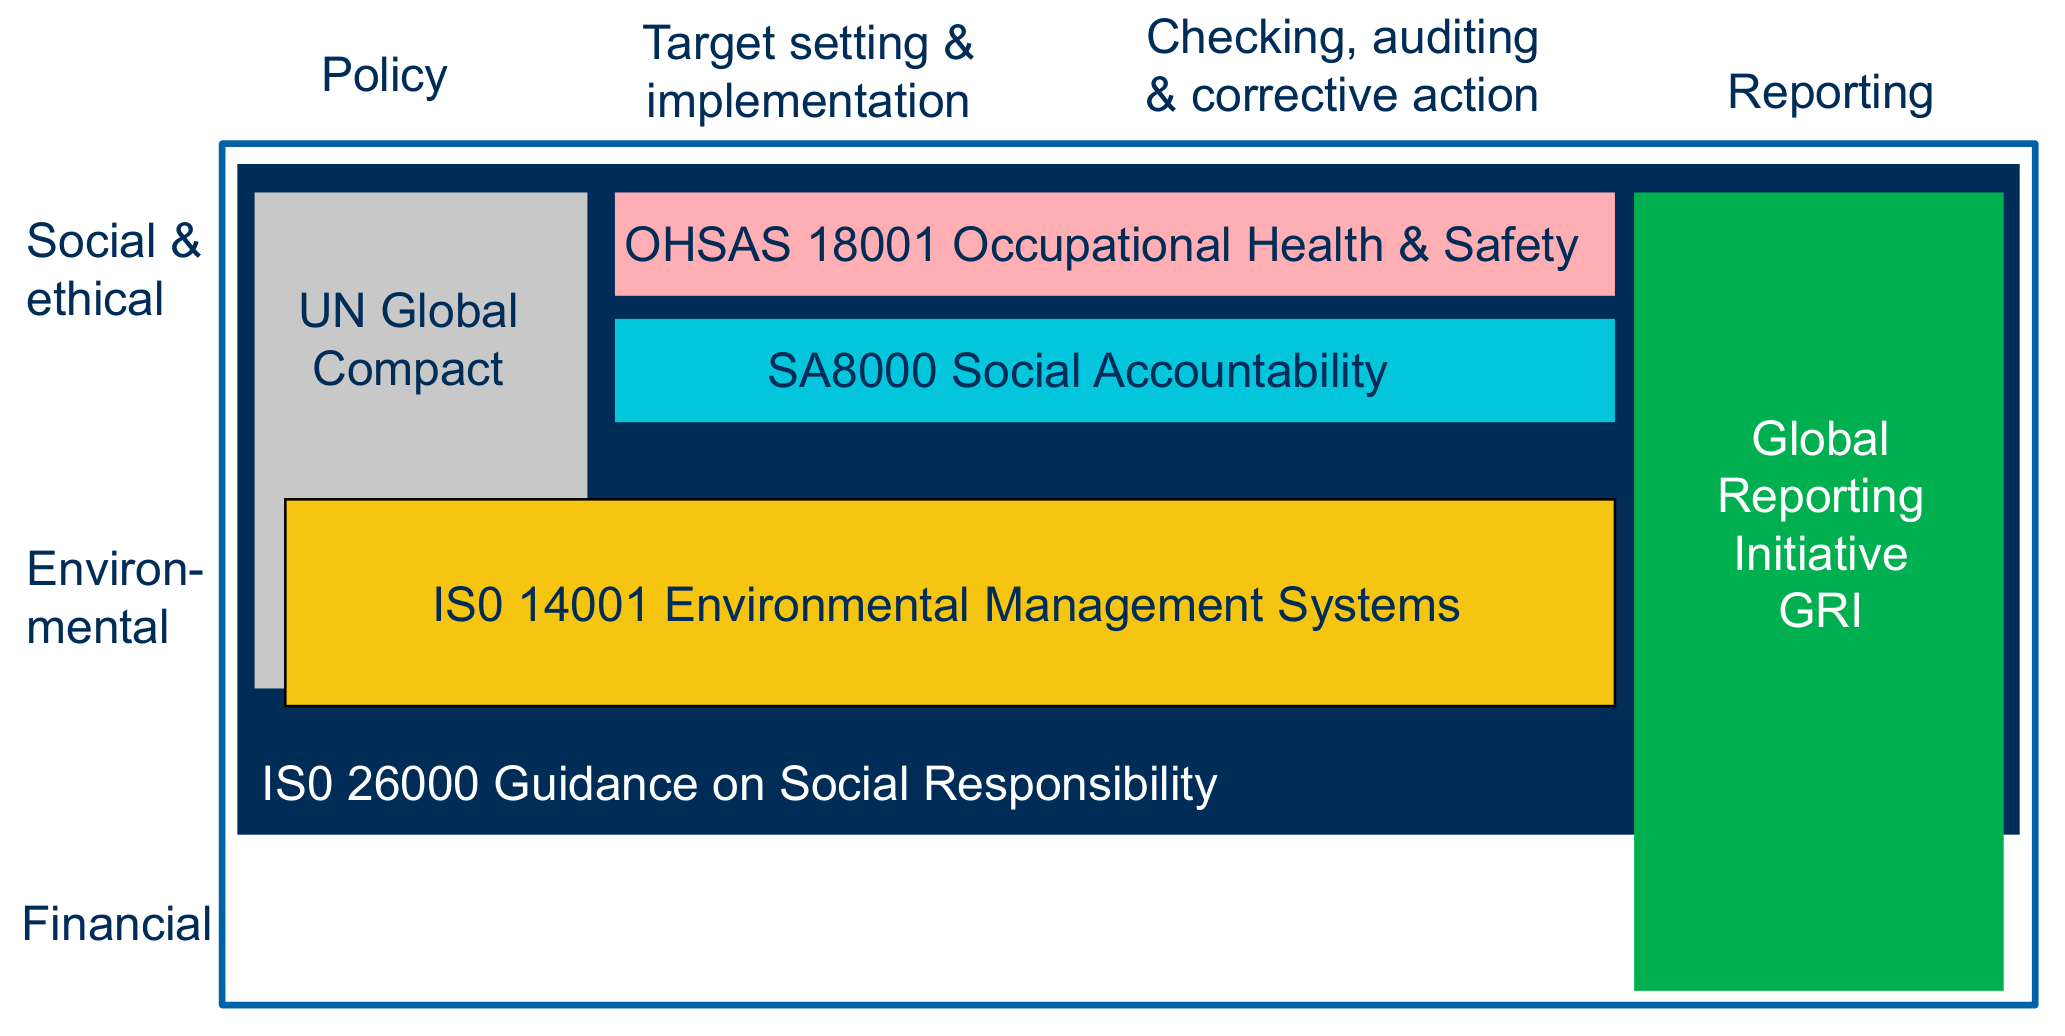
\includegraphics[width=0.8\linewidth]{img/corporate_responsibility_standards}
	\caption{Organisation-related Corporate Responsibility Standards}
	\label{fig:corporateresponsibilitystandards}
\end{figure}

%TODO Check if formatting is still fine
\clearpage
\section{Stakeholder Identification}
\begin{definition}
	A \textbf{business case} is a Forecast of the consequences of an action or decision for the achievement of the highest corporate objective.
\end{definition}

Corporate responsibility requires the use of resources, which must be managed carefully by a competitive company. Thus corporate responsibility must therefore be supported by a business case.

\vspace{1em}
\noindent
\begin{minipage}{0.35\linewidth}
	\centering
	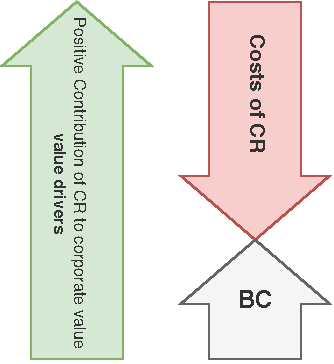
\includegraphics[width=\linewidth]{img/CR_difficulties.pdf}
\end{minipage}
\hfill
\begin{minipage}{0.6\linewidth}
	\textbf{Problem}\\ Value drivers are much more difficult to measure and express in monetary units than costs, and Business Cases are always approximations.
\end{minipage}

\subsection{Value Drivers Which Improve Companies Financial Performance}
\begin{enumerate}
	\item Maintaining a good corporate reputation or brand equity
	\item Attracting, motivating and retaining talented employees
	\item Meeting societal expectations for good corporate behaviour
	\item Improving operational efficiency or decreasing costs
	\item Opening new growth opportunities
	\item Improving risk management
	\item Strengthening competitive position
	\item Improving access to capital
\end{enumerate}
Source: McKinsey \& Company (2009); McKinsey Global Survey Results: Valuing corporate social responsibility

\subsection{Categories of Value Drivers}
\subsubsection{Market–Product–Customers}
Corporate responsibility issues can give rise to the development of new products, technologies, and services, or the upgrading of existing products, technologies, and services. This capacity for innovation can open new markets or customer segments. In this way, a better market position and higher sales volumes or prices can be sought.

\subsubsection{Production–Process–Resources}
Consideration of corporate responsibility issues with regard to the optimization of processes can lead to better quality of work, better social benefits, and better protection for employees. This type of value proposition leads to greater employee satisfaction, increased motivation, and higher productivity. Operational efficiency is increased by the above factors, and costs fall as a result.

\subsubsection{Reputation–Regulation–Public Image}
The reputation of a company is significantly influenced by how it handles stakeholder expectations. If it is sensitive to expectations in relation to corporate responsibility issues, fulfils these wholly or in part, and publicizes its efforts, this will help to preserve its license to operate. Conversely, loss of reputation can lead to high recovery costs.

\subsubsection{Finance-Risk}
A systematic approach to corporate responsibility issues reduces associated risks. Therefore, the risk position of the company from an investor perspective is improved. Thanks to a better risk position, the company has easier access to its own and borrowed capital.

\subsubsection{Conclusion}
\begin{itemize}[label=-]
	\item Corporate responsibility activities need to suit to the company: should be pursued in the way \textbf{most appropriate to each company's strategy and situation}
	\item Corporate responsibility management can be positive or negative for company performance\\It is \textbf{more likely to be profitable, if actively linked to value drivers}, which include \textbf{product innovation, efficiency, reputation, and access to capital}
	\item Benefit of Business Case of corporate responsibility \textbf{is often difficult to quantify}, but it is possible in many cases and should be done much more often
\end{itemize}

\subsection{Management of Corporate Responsibility}
\begin{figure}[H]
	\centering
	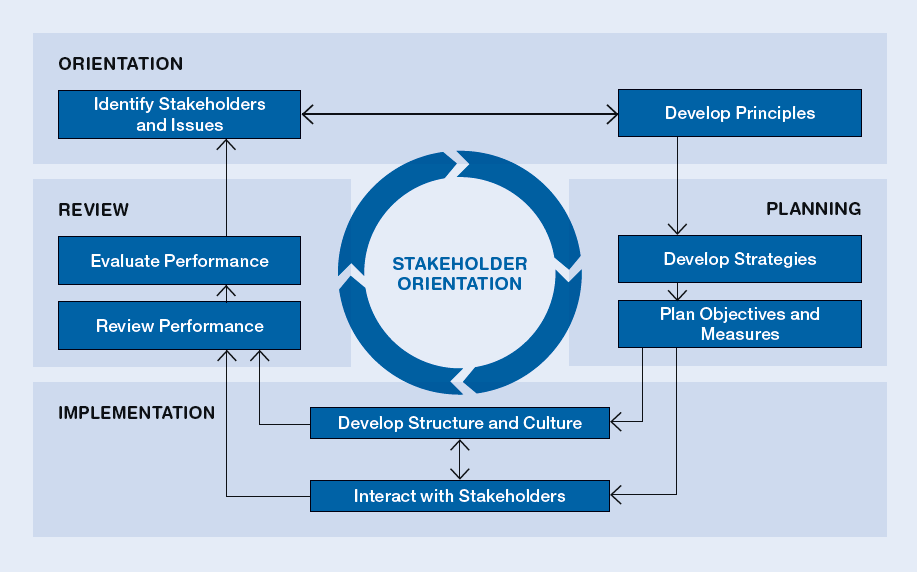
\includegraphics[width=0.8\linewidth]{img/stakeholder_management}
	\caption{Cycle of stakeholder management}
	\label{fig:stakeholdermanagement}
\end{figure}

\begin{definition}
	A \textbf{stakeholder} is any group or individuals that are affected or can affect the achievements of an
	organisation's objective
\end{definition}

\subsection{Stakeholder Theory Approaches}
\begin{itemize}
	\item \textbf{Instrumental}\\
	Looks at stakeholders as means to improve corporate performance
	\item \textbf{Normative}\\
	Looks at stakeholders as ends, individuals or groups with legitimate rights towards the company
	\item \textbf{Descriptive}\\
	Analyses the nature and scope of the various relationships with the stakeholders
\end{itemize}
\parencite{donaldson1995stakeholder}

\subsection{Criteria for Stakeholder Identification}
\begin{itemize}[label=-]
	\item \textbf{Formal and Informal Agreements}\\
	Contracts with employees, performance agreements with suppliers
	\item \textbf{Influence on Corporate Goal Achievement}\\
	Major shareholders by virtue of voting rights, an authority by granting or withdrawing an operating licenses, representatives of influential trade unions
	\item \textbf{Similar Interests to the Company}\\
	Industry associations for collective representation of interests
	\item \textbf{Direct Vicinity to Production Sites}\\
	Entities receiving sponsorship, groups affected by the company
	\item \textbf{Dependence on Company}\\
	Customers whose life depends on the company, employees of major suppliers
\end{itemize}

\subsection{Criteria for the Characterisation and Prioritisation of Stakeholders}
\begin{itemize}
	\item \textbf{Influence}\\
	Ability to enforce its interests, control of key resources, potential to harm the company
	\item \textbf{Organisational Skills}\\
	Ability to create and maintain networks and coalitions
	\item \textbf{Suggestibility}\\
	Availability, willingness to talk, goodwill towards the company
	\item \textbf{Legitimacy}\\
	Entitlement to expectations
	\item \textbf{Urgency}\\
	Time horizon of expectations and demands
	\item \textbf{Interests}\\
	Knowledge of the company, affinity to the company
	\item \textbf{Variety of Perspectives}\\
	Ability to introduce new perspectives or open up new possibilities
\end{itemize}

\begin{figure}[H]
	\centering
	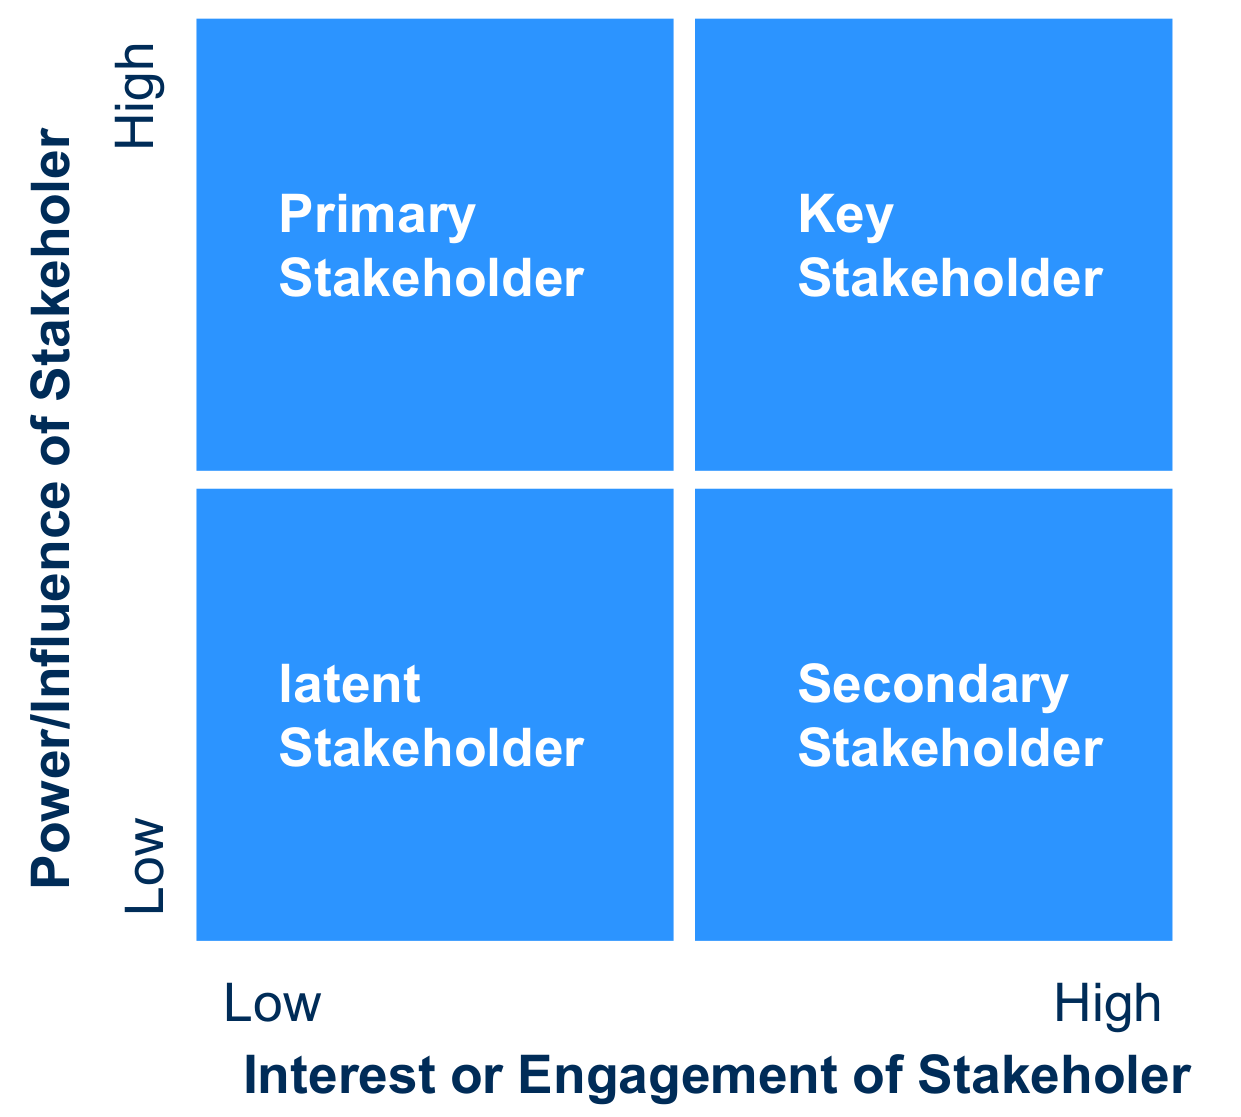
\includegraphics[width=0.5\linewidth]{img/corporate_responsibility_stakeholder_prioritisation}
	\caption{Relevance matrix to classify stakeholders \parencite{winistorfer2012management}}
	\label{fig:corporateresponsibilitystakeholderprioritisation}
\end{figure}

\subsection{Stakeholder Expectations}
The goal is to know the expectations of all or at least the most important stakeholders of the company regarding possible corporate responsibility topics as well as possible, regardless of importance and feasibility. This can be achieved by surveying stakeholders directly, or through interviewing experts who know the stakeholders.

\vspace*{1em}
\noindent
\textbf{Generic Stakeholder Expectations}
\begin{tabularx}{\linewidth}{p{0.26\linewidth} X}
	\cellcolor{DodgerBlue1!40} \textbf{Stakeholder Group} & \cellcolor{DodgerBlue1!40} \textbf{Expectations}\\
	\textbf{Employees} & Salary, job security, status, social environment, meaningful work\\
	\textbf{Management} & Control and power, salary and bonuses, status and prestige, competencies\\
	\textbf{Shareholders} & Control and power, value increase and dividends, tax rate, information\\
	\textbf{Clients} & Quality, value for money, conditions, image, delivery reliability, flexibility\\
	\textbf{Suppliers} & Payment behaviour, acceptance security, image\\
	\textbf{Financial Institutions} & Creditworthiness, power, calculable risk\\
	\textbf{NGOs} & Job preservation, donations and sponsoring, high social or ecological performance, adherence to ethical values\\
	\textbf{State} & Taxes and fees, legal conformity, relief from tasks\\
\end{tabularx}

\section{Topic Prioritisation, Vision and Mission}
The goal is to know the expectations, regardless of importance and feasibility, of stakeholders, ranked by their importance to the company. This can be done by surveying stakeholders directly or by interviewing experts who know the stakeholders.

\vspace{1em}
\noindent
\textbf{Key Questions to Ask}
\begin{itemize}[label=-]
	\item What issues are important to our stakeholders?
	\item What are the topics related to which the company has the highest impact on stakeholders and/or nature?
	\item What issues are our competitors concerned with?
	\item What topics are being covered in the media?
	\item What topics affect (sub-) suppliers or (end-) customers across the whole value chain?
	\item What issues are the subject of (current and future) laws and other mandatory standards?
	\item What topics are the subject of (current and future) voluntary standards; Sustainability Accounting Standard Board (SASB)?
	\item What topics are considered to be significant according to the findings of future and trend analyses?
\end{itemize}

\begin{figure}[H]
	\centering
	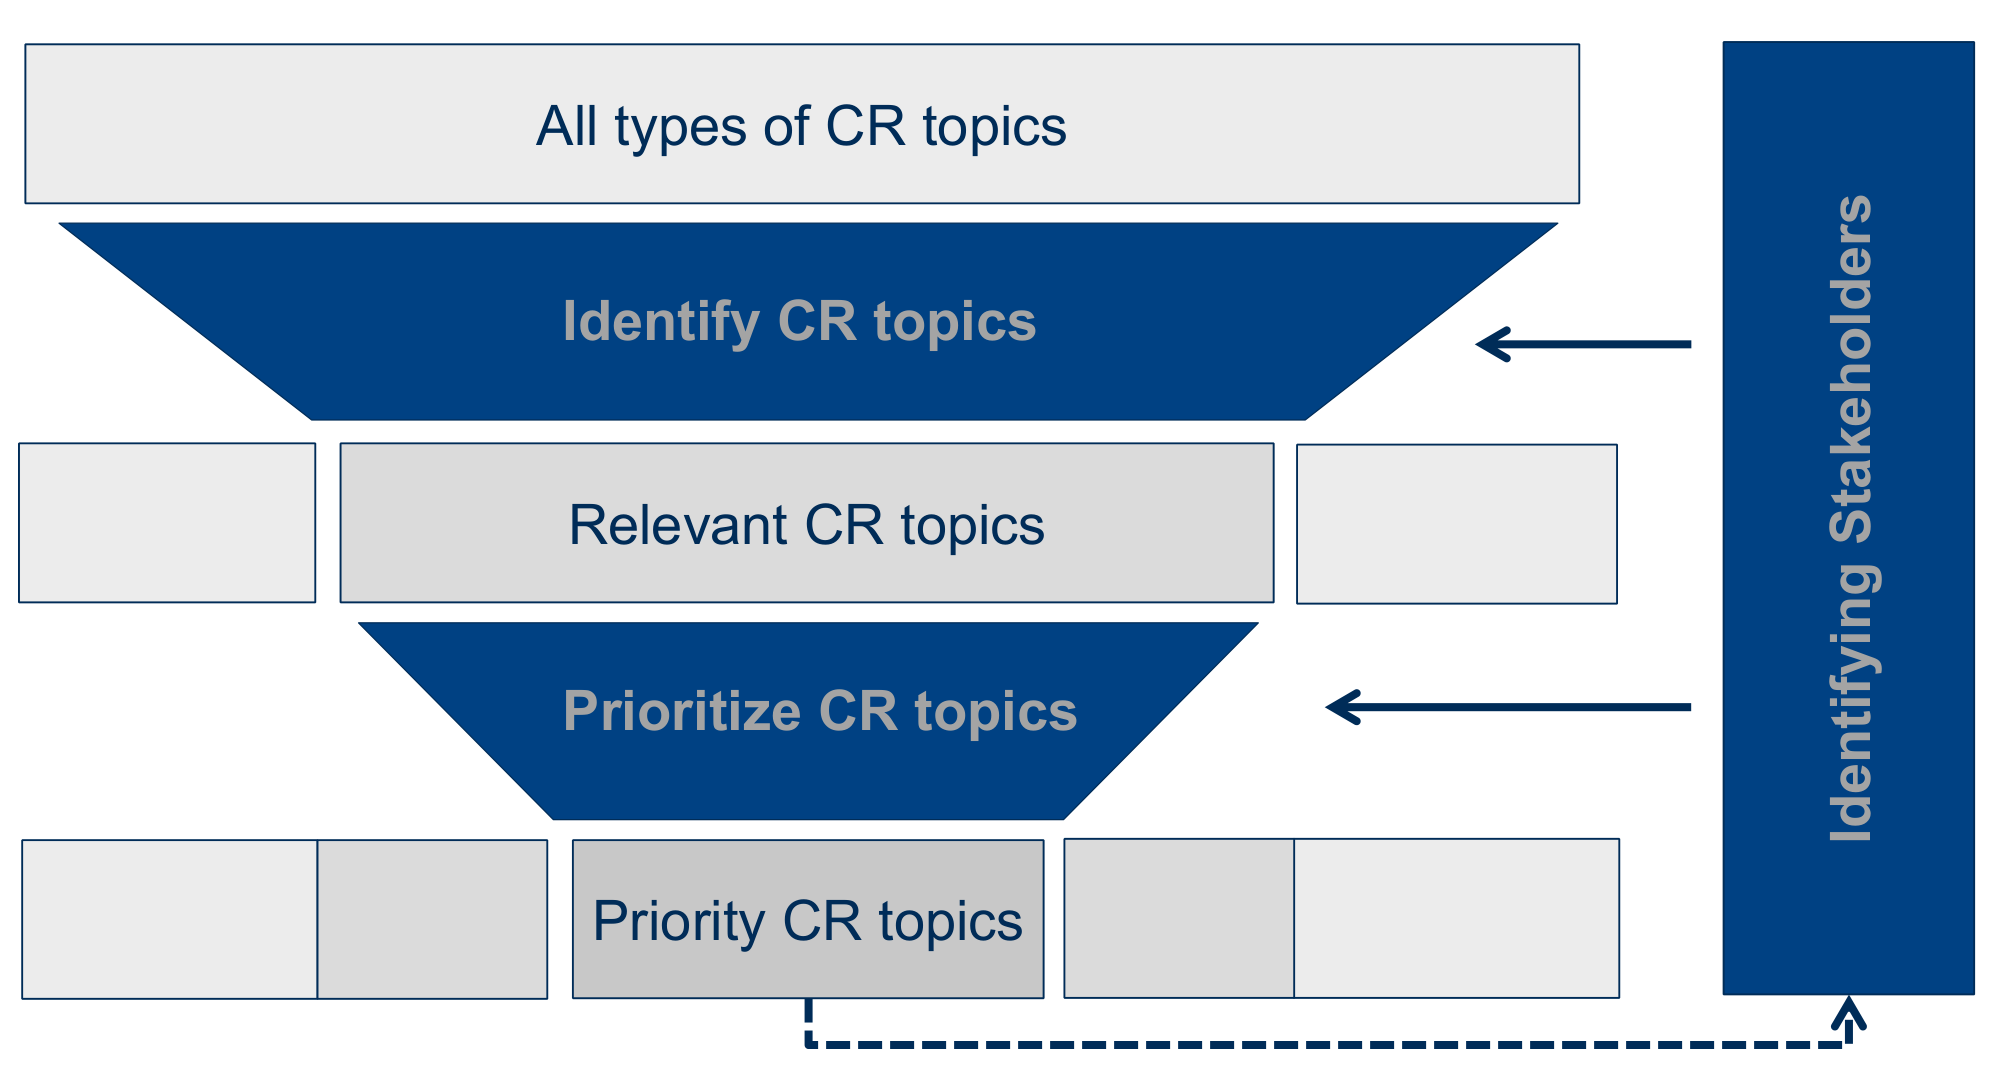
\includegraphics[width=0.6\linewidth]{img/corporate_responsibility_topic_selection}
	\caption{Method of identifying stakeholder key corporate responsibility topics}
	\label{fig:corporateresponsibilitytopicselection}
\end{figure}

\subsection{Topic Identification}
\begin{itemize}[nosep]
	\item Analysis of stakeholder expectations
	\item Analysis of competitors: What topics do they work on?
	\item Analysis of the media landscape
	\item Analysis of the value chain: Which topics concern suppliers, sub-suppliers, customers?
	\item Analysis of binding legal provisions (environmental law, labour law)
	\item Analysis of voluntary standards (ISO 26000, GRI)
	\item Analysis of future studies and long-term trends
\end{itemize}

\subsubsection{Criteria for Topic Prioritisation}
\begin{tabularx}{\linewidth}{X p{0.7\linewidth}}
	\textbf{Dimension} & \textbf{Key Questions}\\
	\hline
	\textbf{Subject Dimension} & \begin{itemize}
		[
			left=0pt,
			nosep,
			before={\begin{minipage}[t]{\hsize}},
			after={\end{minipage}}
		]
		\item How and to what extent are the company's locations, products, activities, business units or processes affected by the topic?
		\item How strong are the company's possibilities to influence the topic?
		\item How significant is the potential for public attention and controversial discussions related to the topic?
		\item What links can be established between the topic and the strategic orientation of the company?
	\end{itemize}\\
	\textbf{Actor Dimension} & How strongly are influential stakeholders interested in the topic?\\
	\textbf{Time Dimension} & Will the importance of the topic increase or decrease in the future?
\end{tabularx}

\begin{definition}
	\textbf{Materiality} is understanding and prioritising the corporate responsibility issues that matter most to our business and stakeholders enables to focus on the right issues and report on them effectively and transparently.
\end{definition}

\noindent
\begin{quote}
	"Materiality is like packing a backpack for a hike: you can only bring the supplies that are absolutely critical, otherwise the weight will slow you down and eventually bring you to your knees."\\
	\hspace*{1em} - Gary Niekerk, Director Global Citizenship, Intel Corporation
\end{quote}

\subsubsection{Determination of Material Topic}
An integrated report should disclose information about matters that substantively affect the \textbf{organisation's ability to create value over the short, medium and long term}. This is determined by considering their effect on the organization's strategy, governance, performance or prospects. Understanding of the perspectives of key stakeholders is critical to identifying relevant matters.

\begin{figure}[H]
	\centering
	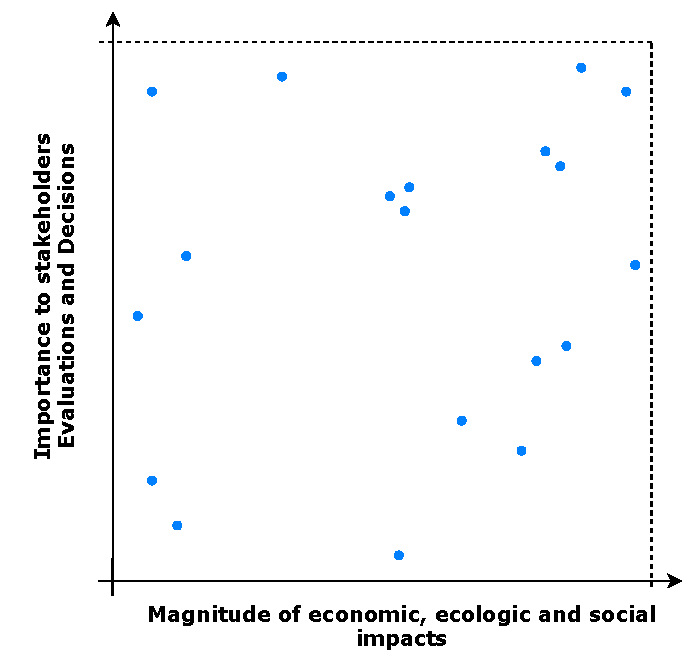
\includegraphics[width=0.6\linewidth]{img/materiality_matrix}
	\caption{Diagram of a sample materiality matrix}
\end{figure}


\begin{tabularx}{\linewidth}{l p{0.7\linewidth}}
	\textbf{Life cycle of a topic} & \\[0.5em]
	\hline
	\textbf{Phase} & \textbf{Characteristics}\\
	\hline
	Latent & \begin{itemize}
		[
			left=0pt,
			nosep,
			before={\begin{minipage}[t]{\hsize}},
			after={\end{minipage}}
		]
		\item Single events indicate a topic
		\item Some Stakeholders bring up a topic
	\end{itemize}\\
	Emerging & \begin{itemize}
		[
			left=0pt,
			nosep,
			before={\begin{minipage}[t]{\hsize}},
			after={\end{minipage}}
		]
		\item Stakeholder expectations are clearly expressed from various sources in connection with the topic
	\end{itemize}\\
	Consolidating & \begin{itemize}
		[
			left=0pt,
			nosep,
			before={\begin{minipage}[t]{\hsize}},
			after={\end{minipage}}
		]
		\item The topic is recognized as such
		\item The need for action becomes apparent
		\item Options for action are examined
	\end{itemize}\\
	Institutionalised & \begin{itemize}
		[
			left=0pt,
			nosep,
			before={\begin{minipage}[t]{\hsize}},
			after={\end{minipage}}
		]
		\item The handling of the topic is established
		\item The chosen solutions are widely accepted and work
	\end{itemize}
\end{tabularx}

\subsection{Important Categories to form a Corporate Culture}
\begin{tabularx}{\linewidth}{l X p{0.4\linewidth}}
	\textbf{Category} & \textbf{Definition} & \textbf{Leading Questions}\\
	\hline
	Values & Basic values with general principles of conduct such as leadership, participation and cooperation. & \begin{itemize}
		[
			left=0pt,
			nosep,
			before={\begin{minipage}[t]{\hsize}},
			after={\end{minipage}}
		]
		\item What is important to us in our work?
		\item What should guide our actions?
	\end{itemize}\\
	Mission & Description of corporate purpose, value proposition for key stakeholders, core competencies and strategic value proposition. & \begin{itemize}
		[
		left=0pt,
		nosep,
		before={\begin{minipage}[t]{\hsize}},
			after={\end{minipage}}
		]
		\item What makes our company special?
		\item What is our purpose?
	\end{itemize}\\
	Vision & Long-term conception of the desired future & \begin{itemize}
		[
		left=0pt,
		nosep,
		before={\begin{minipage}[t]{\hsize}},
			after={\end{minipage}}
		]
		\item Where will our company be in 5 to 10 years?
		\item Where are we heading?
	\end{itemize}
\end{tabularx}

\begin{figure}[H]
	\centering
	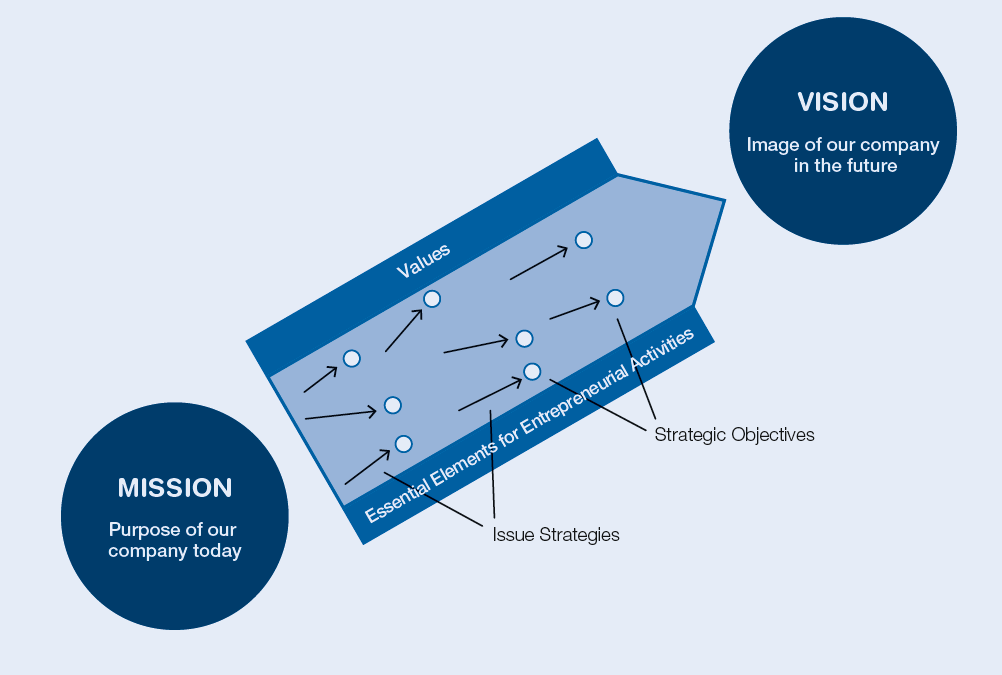
\includegraphics[width=0.7\linewidth]{img/interaction_mission_strategy_issues}
	\caption{Interaction between mission statement, strategic objectives and issue strategies}
	\label{fig:interactionmissionstrategyissues}
\end{figure}

\section{Corporate Responsibility Strategies}
As can be seen in figure \ref{fig:interactionmissionstrategyissues} the strategies are the guiding principle on how a company gets from its current mission to the future state envisioned by management and stakeholders. Strategies are not just created and then implemented, they have to be managed and adapted to changing circumstances.

\begin{tabularx}{\linewidth}{p{0.5\linewidth} X}
	\multicolumn{2}{c}{\textbf{Strategic Corporate Responsibility Management}}\\
	\multicolumn{2}{c}{creates value for the ..}\\[0.5em]
	\textbf{Society and Environment} & \textbf{Company}\\[0.5em]
	\begin{itemize}
		[
		left=0pt,
		nosep,
		before={\begin{minipage}[t]{\hsize}},
			after={\end{minipage}}
		]
		\item Climate change mitigation
		\item Safeguarding human rights in the supply chain
		\item Endangered biomes protection
		\item etc.
	\end{itemize} & Contributes to \textbf{Company Value} and \textbf{Success}: business case, value drivers, creating shared value
\end{tabularx}

\subsection{Perspective on Business Cases of Corporate Responsibility}
\begin{tabularx}{\linewidth}{p{0.5\linewidth} X}
	\textbf{Benefit Fields} & \textbf{Value Drivers}\\
	\hline
	Market-Product-Customer & Product innovation and differentiation\\
	Production-Process-Resources & Process innovation, Efficiency, Securing of resources\\
	Reputation-Regulation-Public & Reputation and public opinion\\
	Finance-Risk & Risk position and access to capital
\end{tabularx}

\subsection{Fields of Strategic Management}
\begin{tabularx}{\linewidth}{p{0.5\linewidth} p{0.5\linewidth}}
	\multicolumn{2}{l}{\textbf{Corporate Strategy}}\\
	\multicolumn{2}{l}{$\bullet$ Competitive strategy (quality versus cost)}\\
	\multicolumn{2}{l}{$\bullet$ Market strategy (regional versus global)}\\
	\multicolumn{2}{l}{$\bullet$ Financing strategy (proprietary capital versus borrowed capital)}\\[0.5em]
	\textbf{Functional Strategies} & \textbf{Issue Strategies}\\
	\begin{itemize}
		[
		left=0pt,
		nosep,
		before={\begin{minipage}[t]{\hsize}},
			after={\end{minipage}}
		]
		\item HR Strategy
		\item Research and Development Strategy
		\item Corporate Responsibility Strategy
	\end{itemize} & \begin{itemize}
		[
		left=0pt,
		nosep,
		before={\begin{minipage}[t]{\hsize}},
			after={\end{minipage}}
		]
		\item Climate Change Mitigation Strategy
		\item Human Rights Strategy
		\item Employee Training Strategy
	\end{itemize}
\end{tabularx}

\begin{definition}
	A \textbf{strategy} is a consistent collection of activities that distinguishes an enterprise from its competitors.
\end{definition}
\begin{definition}
	Issues are considered as \textbf{strategic} if they have a sustainable effect on the success and success potential of an enterprise.
\end{definition}
\begin{definition}
	\textbf{Strategic management} is the creation, management, and development of the success of an enterprise.
\end{definition}
\begin{definition}
	\textbf{Corporate responsibility strategy} is the manner how and the degree to which a company connects corporate responsibility activities with company success.
\end{definition}

%TODO Check if formatting is still fine
\clearpage
\subsection{Basic Types of Corporate Responsibility Strategies}
\begin{tabularx}{\linewidth}{m{1.5em} >{\centering}m{1em} >{\centering}m{4cm} >{\centering\arraybackslash}m{4cm}}
	& & \multicolumn{2}{c}{\textbf{Sustainability Strategies}}\\
	& & \multicolumn{2}{c}{Existing Markets}\\
	\multirow{2}{*}[2em]{\rotatebox{90}{\textbf{Competitive Advantage}}} & \rotatebox{90}{Lower Costs} & \cellcolor{DarkSeaGreen3} Eco-Efficiency & \cellcolor{SpringGreen3} Environmental Cost Leadership\\
	& \rotatebox{90}{Differentiation\hspace*{1em}} & \cellcolor{SeaGreen2} Beyond Compliance Leadership & \cellcolor{DarkSeaGreen1} Eco-Branding\\
	& & Processes & Products and Services\\[0.5em]
	& & \multicolumn{2}{c}{\textbf{Competitive Focus}}
\end{tabularx}

\begin{itemize}
	\item \textbf{eco-efficiency} is doing more with less and lower environmental impact. This can lead to breakthrough innovations and improvements in resource utilisation, because applying Lean Thinking to operations management, waste and by-products, can eventually be converted to new sources of income
	\item \textbf{beyond compliance leadership} requires that companies go above and beyond what their competitors are doing
	\item \textbf{eco-branding} involves finding a point of differentiation based on the ecological characteristics of certain products; that is Labels such as FSC, MSC; Bio-Knospe
	\item \textbf{environmental cost leadership} entails selling products with good environmental performance but with an equally attractive price proposition
\end{itemize}

%TODO Check if formatting is still fine
\clearpage
\subsection{Approach for a Corporate Responsibility Strategy: Leader or Follower}
\begin{tabularx}{\linewidth}{>{\raggedright}p{0.3\linewidth} >{\raggedright}p{0.32\linewidth} >{\raggedleft\arraybackslash}p{0.32\linewidth}}
	& \cellcolor{SteelBlue1!75} \textbf{FOLLOWER} & \cellcolor{SteelBlue1!75} \textbf{LEADER}\\
	& \cellcolor{SteelBlue1!75} Defensive and Risk-oriented & \cellcolor{SteelBlue1!75} Offensive and Opportunity-oriented\\
	& \cellcolor{SteelBlue1!75} Low CR performance & \cellcolor{SteelBlue1!75} High CR performance\\[1em]
	\cellcolor{DodgerBlue1!25} \textbf{Perspective} & \cellcolor{DodgerBlue1!25} Example Strategic Objectives & \cellcolor{DodgerBlue1!25} Example Strategic Objectives\\[1em]
	\cellcolor{DodgerBlue1!25} \textbf{Market-Product-Customer} & Safeguard existing market position & Develop new markets or market segments through product innovation\\[1em]
	\cellcolor{DodgerBlue1!25} \textbf{Production-Process-Resources} & Focus on business continuity, securing supply chain, ensure cost savings and efficiency, reduced absenteeism & Reward process innovation, recruit top talent\\[1em]
	\cellcolor{DodgerBlue1!25} \textbf{Reputation-Regulation-Public} & Reputation protection, secure license-to-operate & Reputation and brand building, proactive preparedness for restrictive legislation\\[1em]
	\cellcolor{DodgerBlue1!25} \textbf{Finance-Risk} & Reduce risk, secure access to capital & Develop access to new forms of capital\\[1em]
\end{tabularx}
Investors are mainly focussed on economic indicators, but sustainability rankings by sustainability rating agencies can be a decisive factor in investment decisions, if two companies are economically at a comparable level.

\subsection{Shared Value Approach}
The reaction of companies to societal challenges is often cosmetic, not strategic or substantial. However, the Corporate Responsibility field remains strongly linked with a moral imperative (absolute), companies in contrast need to balance competing interests and costs (relative). The Sustainability field \textbf{offers little to balance long-term objectives and short-term costs}. The Creating Shared Value (CSV) approach tries to bridge economy and society.

\begin{quote}
	\textquotedblleft Not all profit is equal. Profits involving a social purpose represent a higher form of capitalism, one that creates a positive cycle of company and community prosperity.\textquotedblright
\end{quote}

\begin{definition}
	\textbf{Creating shared value} involves policies and operating practices that enhance the competitiveness of a company while simultaneously advancing the economic and social conditions in the communities in which it operates \parencite{kramer2011creating}.
\end{definition}

\vspace*{1em}
\noindent
The CSV approach works by \textbf{integration of a social perspective into the core framework} the company already uses to understand competition and guide its business strategy. \textbf{Creating a social dimension to the value proposition},  \textbf{identification of social dimensions} of a company’s competitive context, and \textbf{defining customers' needs}. It directly links to the company value creation and profit maximization. This strategic approach is very specific to the company to differentiate in the market and to choose a unique position.

\subsubsection{Methods}
\begin{itemize}
	\item \textbf{Rethink Products and Markets}\\
	Identify all the societal needs, benefits, and harms that are or could be embodied in the firm’s products, which leads to new product innovations
	\item  \textbf{Redefine Productivity in the Value Chain}\\
	Congruence between societal progress and productivity: better efficiency, securing of resources
	\item \textbf{Enable Local Cluster Development}\\
	Geographical concentrations of firms, related businesses, suppliers, service providers and logistical infrastructure
\end{itemize}

\subsubsection{Benefits}
Socially and environmentally, shared value can vastly improve the conditions of a society, advancing community health, education, employment, service access and participation, and helping to conserve wildlife and environments. The economic benefits for a company granted by shared value are also numerous, and include, but are not limited to:
\begin{itemize}[label=-, nosep]
	\item Self-sustaining purpose and profitability
	\item Stronger brand equity and marketability
	\item Increased customer preference and loyalty
	\item Higher advocacy, retention and productivity among employees
	\item Resilience against external business threats
	\item Regained credibility among a disillusioned public
	\item Enhanced or sustained interest from like-minded shareholders and investors
\end{itemize}
\section{Corporate Responsibility Goal Setting}
\citeauthor{stead2008sustainable} base their approach on the works of early business management scholars like Taylor 

\subsection{Plan Objectives and Measures}
Operational objectives are \textbf{specific short to medium term goals}, which are \textbf{derived from the strategic objectives}. They \textbf{make these strategic objectives measurable and verifiable}, and thus serve as a guide in the implementation phase. They are required to be \textbf{s}pecific, \textbf{m}easurable, \textbf{a}ccepted, \textbf{r}ealistic and \textbf{t}ime-based.

\begin{tabularx}{\linewidth}{p{0.2\linewidth} X}
	\cellcolor{DodgerBlue1!40}& \cellcolor{DodgerBlue1!40}\\
	\cellcolor{DodgerBlue1!40} \textbf{Requirement} & \cellcolor{DodgerBlue1!40} \textbf{Description}\\
	\cellcolor{DodgerBlue1!40}& \cellcolor{DodgerBlue1!40}\\
	\textbf{Specific} & formulated in a clear, straightforward and detailed manner\\[1em]
	\textbf{Measurable} & describe a result that is verifiable by means of indicators \\[1em]
	\textbf{Accepted} & accepted by the people responsible for achieving the objectives\\[1em]
	\textbf{Realistic} & formulated in a way that makes their achievement realistic\\[1em]
	\textbf{Time-Based} & have a date which establishes the point of completion
\end{tabularx}

\begin{tabularx}{\linewidth}{p{0.2\linewidth} X}
	\cellcolor{DodgerBlue1!40} \textbf{Levels} & \cellcolor{DodgerBlue1!40} \textbf{Strategic Objective: \textquotedblleft In ten years, we will be the industry leader when it comes to the proportion of women in management positions \textquotedblright}\\
	\textbf{Principles} & Within two years, all sites will have adopted gender equality into their human resources policy\\
	\textbf{Processes} & In the coming year, at each location, a minimum of 20 female participants will have taken part in the mentoring program\\
	\textbf{Effects} & Within three years, the percentage of women in lower and middle management will have increased across all locations by 20\% compared to the base value target date\\
\end{tabularx}

\subsection{Relevance of Indicators in the Measurement of Objectives}
Indicators are necessary to measure the achievement of objectives and need to be defined for the operational objectives. A corporate responsibility indicator can be defined as information which characterises the performance of organizations regarding a particular corporate responsibility issue. These indicators must be collected at regular intervals. Indicators can also be used at different organisational levels.
\begin{tabularx}{\linewidth}{p{0.2\linewidth} X}
	\cellcolor{DodgerBlue1!40} \textbf{Levels} & \cellcolor{DodgerBlue1!40} \textbf{Example Issue: Women in Management Positions}\\
	\textbf{Principles} & Percentage of locations that have added gender equality to their HR policy in \%\\
	\textbf{Processes} & Number of women per location and year who have completed a mentoring program\\
	\textbf{Effects} & Proportion of women in lower and middle management across all locations in \%\\
\end{tabularx}


\subsection{Indicator Types}
\begin{tabularx}{\linewidth}{p{0.3\linewidth} X X}
	\multicolumn{2}{c}{\cellcolor{DodgerBlue1!40} \textbf{Indicator Type}} & \cellcolor{DodgerBlue1!40} \textbf{Characteristics}\\
	\multirow{3}{*}{\textbf{Qualitative Indicators}} & Binary Indicators & Two description states (yes/no, available/not available, true/false)\\
	& Graduated Indicators & Several possible states (not at all/somewhat/much/very much)\\
	& Descriptive Indicators & Description of issues in written form\\
	\multirow{2}{*}{\textbf{Quantitative Indicators}} & Absolute Indicators & Numerical values without references variables\\
	& Relative Indicators & Numerical values with references variables\\
\end{tabularx}

%TODO Check if formatting is still fine
\clearpage
\subsection{Developing Measures}
To achieve the operational objectives of corporate responsibility issues, specific measures need to be developed. This applies to all activities which are carried out to meet objectives, such as adapting processes and structures, or implementing programs and projects.
\begin{figure}[H]
	\centering
	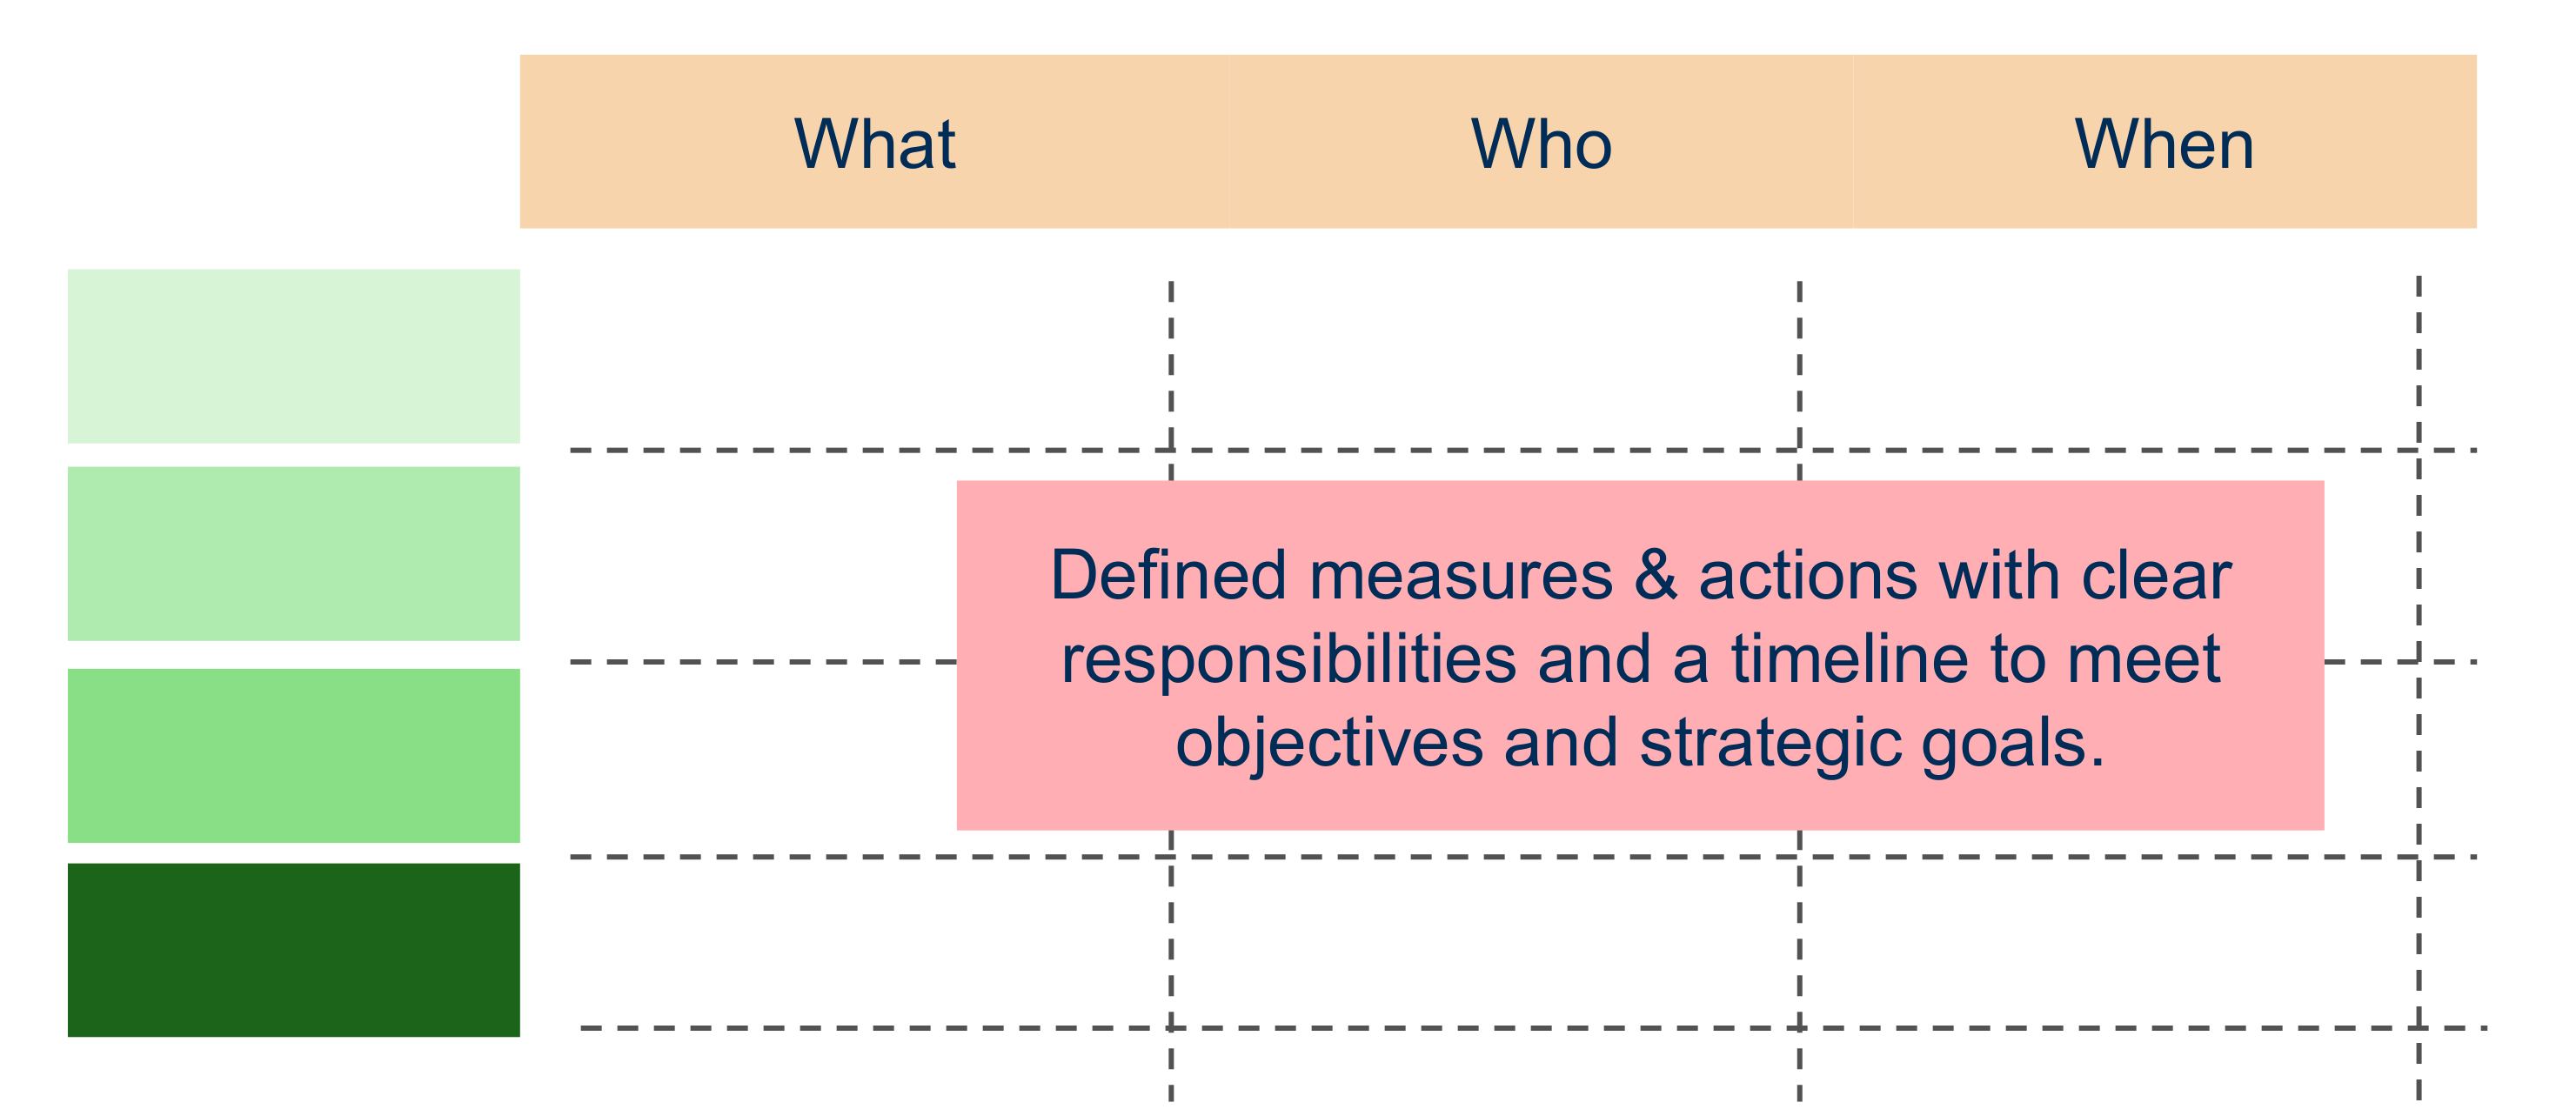
\includegraphics[width=0.7\linewidth]{img/developing_achievable_measures}
	\caption{Matrix to classify and design defined measures to achieve strategic goals}
	\label{fig:developingachievablemeasures}
\end{figure}
Companies need to rethink the way they measure and set goals on environmental and social performance. Current goals are most often set in comparison to their peer group, which makes them very unambitious. Linking sustainability goals to business outcomes is not only vital, it is also very often missing from the storyline. Often times, setting sustainability goals involve too many topics, and are not focussed enough to be meaningful targets. Environmental and social context is also missing from most sustainability targets, resulting in goals that lack sufficient ambition.

\section{Corporate Responsibility Management Structures and Stakeholder Engagement}
\subsection{Implementation of a Corporate Responsibility Strategy}
Key tasks during the implementation phase of corporate responsibility issues are the design of appropriate work structures and the promotion of an enterprise culture. Both are needed to integrate and implement the principles, strategies, objectives, and measures within the company.

\vspace*{0.5em}
\begin{tabularx}{\linewidth}{p{0.4\linewidth} p{0.4\linewidth}}
	\multicolumn{2}{c}{\cellcolor{DodgerBlue1!40} {\large\textbf{Implementing Corporate Responsibility}}}\\[0.5em]
	\textbf{Operational Structure} & \textbf{Organisational Structure} \\[0.5em]
	Designing and describing the processes necessary to perform tasks. & Defining tasks and assigning them to different organizational units. \\[2em]
	\multicolumn{2}{c}{\textbf{Organisational Culture}}
\end{tabularx}

\subsection{Corporate Responsibility Management Tasks}
Central questions are \textit{what tasks have to be fulfilled} and \textit{which units will be in charge of a task}?
\begin{tabularx}{\linewidth}{p{0.45\linewidth} p{0.45\linewidth}}
	\cellcolor{DodgerBlue1!40} \textbf{Task Categories} & \cellcolor{DodgerBlue1!40} \textbf{Examples}\\[1em]
	\textbf{Cross-Cutting Tasks} & \begin{itemize}
		[
		left=0pt,
		nosep,
		before={\begin{minipage}[t]{\hsize}},
			after={\end{minipage}}
		]
		\item Adopt a mission statement
		\item Analyse relevant stakeholders and issues
		\item Coordinate stakeholder dialogue
		\item Develop issue strategies and align them with the corporate strategy
		\item Evaluate performance on issues
		\item Coordinate communication on issues
	\end{itemize}\\
	\textbf{Division-Specific Tasks} & \begin{itemize}
		[
		left=0pt,
		nosep,
		before={\begin{minipage}[t]{\hsize}},
			after={\end{minipage}}
		]
		\item Translate issue strategies into objective with indicators and measures
		\item Implement individual actions and projects related to the issue
		\item Collect data and information for reviewing target achievement
	\end{itemize}
\end{tabularx}

\subsection{Organising Corporate Responsibility Tasks}
Various units are involved in carrying out and reviewing tasks:
\begin{tabularx}{\linewidth}{p{0.3\linewidth} X}
	\textbf{Divisions} & Corporate responsibility issues linked to functions\\
	\textbf{Specialist Department} & Corporate responsibility issues are often interdisciplinary topics which cut across organisational units. This needs to be reflected in these structures. Rather than being entrusted to one division, the responsibility for performance is exercised by a specialist department.\\
	\textbf{Responsible Persons in Different Divisions} & In affected organisational units, individuals are appointed to deal with issues. This can take on various different forms. One person can deal exclusively with corporate responsibility issues, but an individual assumes responsibility for such issues in addition to its other duties.\\
	\textbf{Steering Committees} & Handling of corporate responsibility issues through cross-cutting committees. Their function is to bring together information from the lines and other cross-cutting functions, without substantially altering competencies and responsibilities.\\
	\textbf{Project Teams} & Implementing single and individual corporate responsibility projects.\\
	\textbf{Combining different organisational forms} & A combination of various forms is especially recommended for large organizations. A specialist department acts as a focal point, while a cross-sectional committee coordinates the various tasks between divisions.
\end{tabularx}
\begin{itemize}
	\item Most operational sequences occur repeatedly in a company
	\item Important to achieve a common understanding of these processes,
	\item To achieve such understanding, processes need to be described and explained (e.g. by using diagrams)
	\item Common classifications are management processes, implementation (also core or performance) and support processes.
	\item For corporate responsibility issues, it is often necessary to \textbf{adapt} existing processes or \textbf{introduce} new ones.
\end{itemize}

%TODO Check if formatting is still fine
\clearpage
\subsection{Development of a Corporate Culture for Corporate Responsibility}
\begin{definition}
	A \textbf{corporate culture} is understood as the total number of value convictions, thought patterns and behavioural norms that have been consciously or unconsciously cultivated, symbolically or linguistically handed down in the company, which have developed and proven themselves and which are therefore conveyed to the company's employees as valid forms of perception, thinking, judging, speaking and behaviour. (Schein, 1985 and Ulrich, 1984)
\end{definition}

\begin{tabularx}{\linewidth}{p{0.96\linewidth}}
	\cellcolor{DodgerBlue1!40} \textbf{The Organisational Iceberg}\\[0.5em]
	\begin{itemize}
		[
		left=0pt,
		nosep,
		before={\begin{minipage}[t]{\hsize}},
			after={\end{minipage}}
		]
		\item Organizational specifications
		\item Rules, regulations, manuals
		\item Local and regional specifications
		\item Information Technology specifications
	\end{itemize}\\
	\hline
	\begin{itemize}
		[
		left=0pt,
		nosep,
		before={\begin{minipage}[t]{\hsize}},
			after={\end{minipage}}
		]
		\item Identity, collective expectations, patterns of interpretation and background beliefs
		\item Values and norms
		\item Attitudes in leadership and cooperation within and towards stakeholders
		\item Myths, Legends
		\item Typical argumentation patterns and language rules
	\end{itemize}
\end{tabularx}

\begin{tabularx}{\linewidth}{p{0.22\linewidth} p{0.22\linewidth} p{0.22\linewidth} p{0.22\linewidth}}
	\multicolumn{4}{c}{\cellcolor{DodgerBlue1!40} \textbf{Cultural Change}}\\[0.5em]
	\textbf{Step 1} & \textbf{Step 2} & \textbf{Step 3} & \textbf{Step 4}\\
	\textbf{Information} & \textbf{Creation of Understanding} & \textbf{Commitment} & \textbf{Motivation}\\[1.5em]
	Reporting on the importance and relevance of sustainability issues with comprehensive and tailored information. This is done to build a common language, creating understanding and raising awareness. Acceptance must be supported by top management. & Creating and promoting understanding and a perception of issues. Involves all employees. & Commit employees to tasks and thus control their contribution to the corporate responsibility strategy implementation. & Implementing projects and measures on corporate responsibility topics across all hierarchical levels to create a sense of unity.
\end{tabularx}

\subsection{Influencing Behaviour and Overcoming Resistance}
\begin{itemize}
	\item \textbf{Incentives}\\ Give out bonuses for top achievers of a specific goal
	\item \textbf{Compliance}\\ Draw up a set of regulations which must be signed and complied with on risk of dismissal
	\item \textbf{Integrity}\\ Extensive training of all involved parties, with workshops on the consequence of that specific topic
\end{itemize}

\subsection{Stakeholder Engagement}
The benefits of stakeholder engagement involve
\begin{itemize}
	\item Exchange of knowledge and experience
	\item Gaining an outside view, overcoming operational blindness and narrow focus
	\item Identifying issues early, having an early warning system
	\item Preventing criticism, lifting blockades
	\item Anticipation and development of new solutions
	\item Greater acceptance of decisions and actions through stakeholder involvement in development processes
	\item Improved relationships, building trust
	\item Development of innovative solutions, services and products through cooperation
	\item Building reputation and securing the licence to operate
\end{itemize}

\begin{tabularx}{\linewidth}{p{0.22\linewidth} | p{0.22\linewidth} | p{0.22\linewidth} | p{0.22\linewidth}}
	\multicolumn{4}{c}{\cellcolor{DodgerBlue1!40} \textbf{Forms of Stakeholder Engagement}}\\[0.5em]
	\textbf{Information} & \textbf{Consultation} & \textbf{Dialogue} & \textbf{Partnership}\\[0.5em]
	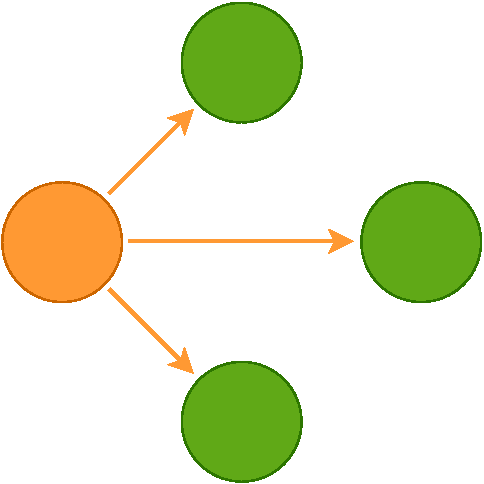
\includegraphics[width=\linewidth]{StakeholderEngagement_Information} & 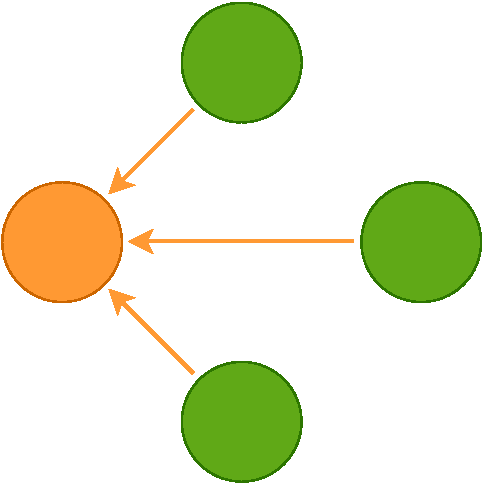
\includegraphics[width=\linewidth]{StakeholderEngagement_Consultation} & 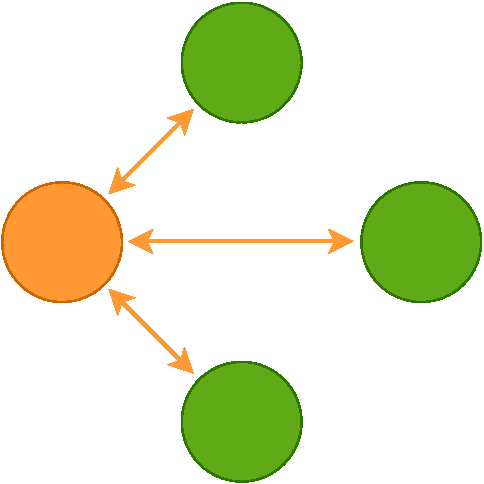
\includegraphics[width=\linewidth]{StakeholderEngagement_Dialogue} & 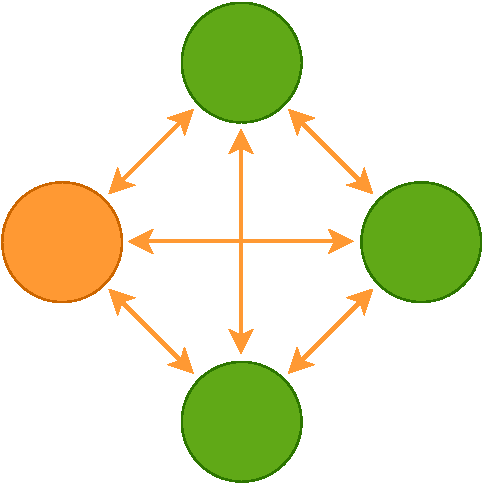
\includegraphics[width=\linewidth]{StakeholderEngagement_Partnership}\\
	Providing Information - \textbf{send} & Perception of attitudes and expectations - \textbf{receive} & Mutual exchange of information - \textbf{send \& receive} & Cooperation to achieve common goals\\[3.5em]
	\begin{itemize}
		[
		left=0pt,
		nosep,
		before={\begin{minipage}[t]{\hsize}},
			after={\end{minipage}}
		]
		\item Homepage
		\item Newsletter
		\item Brochures
		\item Reports
		\item Media Releases
		\item Speeches
	\end{itemize} & \begin{itemize}
	[
	left=0pt,
	nosep,
	before={\begin{minipage}[t]{\hsize}},
		after={\end{minipage}}
	]
		\item Surveys
		\item Online Feedback
		\item Citizens' Consultation
		\item Interviews
	\end{itemize} & \begin{itemize}
	[
	left=0pt,
	nosep,
	before={\begin{minipage}[t]{\hsize}},
		after={\end{minipage}}
	]
		\item Stakeholder Forums
		\item Online Engagement and an Exchange of Ideas
		\item Conferences
		\item Advisory Boards
	\end{itemize} & \begin{itemize}
	[
	left=0pt,
	nosep,
	before={\begin{minipage}[t]{\hsize}},
		after={\end{minipage}}
	]
		\item Local, Sustainable Projects
		\item Multi-stakeholder Initiatives, Round Tables
		\item Alliances
	\end{itemize}
\end{tabularx}

%TODO Check if formatting is still fine
\clearpage
\section{Corporate Responsibility Communication and Controlling}
Communication matters in how transparent and credible the reporting, especially on non-financial topics, is, and how the corporate responsibility activities and communications are perceived by your shareholders.

\begin{tabularx}{\linewidth}{p{0.2\linewidth} p{0.18\linewidth} p{0.16\linewidth} p{0.16\linewidth} X}
	\cellcolor{SteelBlue1!75}\textbf{Name} & \cellcolor{SteelBlue1!75}\textbf{Criteria} & \cellcolor{SteelBlue1!75}\textbf{Description} & \cellcolor{SteelBlue1!75}\textbf{Deliverables} & \cellcolor{SteelBlue1!75}\textbf{Recipients}\\[0.5em]
	\textbf{Global Reporting Initiative} & Indicator-based & Public domain, Voluntary & Report & All Stakeholders\\[2.5em]
	\textbf{International Integrated Reporting Council} & Principle-based & Public domain, Voluntary & Report & All Stakeholders\\[3.5em]
	\textbf{Global Real Estate Sustainability Benchmark} & Indicator-based, focus on industry & Membership, Voluntary & Survey & Investors\\[3.5em]
	\textbf{Principles of Responsible Investment} & Indicator- and Principle-based & Membership, Voluntary & Survey & Investors, Customers\\[3.5em]
	\textbf{UN Global Compact} & Principle-based & Membership, Voluntary & Conference of the Parties (COP) & All Stakeholders\\[3.5em]
	\textbf{EU Directive} & Indicator-based & Obligatory in the EU & Report & All Stakeholders and State Authorities
\end{tabularx}

\subsubsection{Global Reporting Initiative (GRI) Reporting Standards}
The modular, interrelated GRI Standards are designed primarily to be used as a set, to prepare a sustainability report focused on material topics. The three universal Standards are used by every organization that prepares a sustainability report. An organization also chooses from the topic-specific Standards to report on its material topics – economic, environmental or social.

\begin{figure}[H]
	\centering
	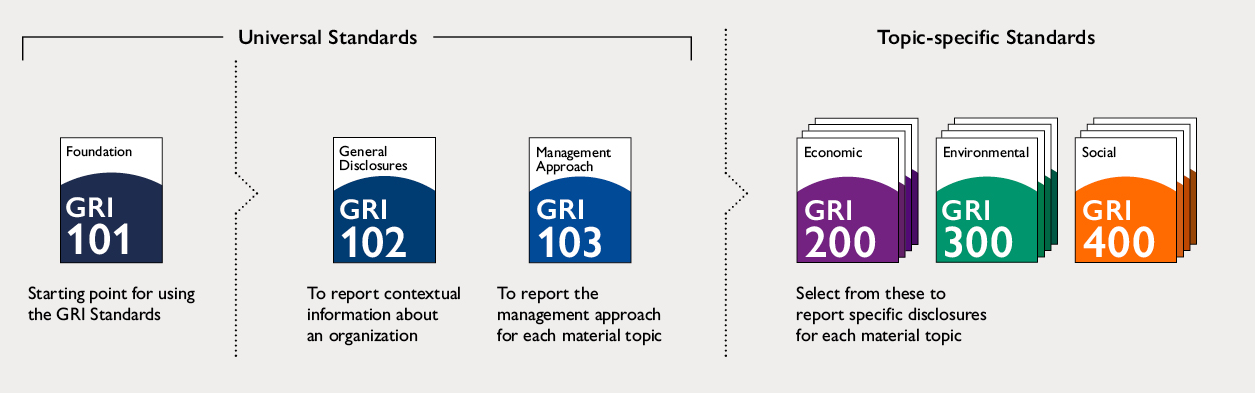
\includegraphics[width=0.9\linewidth]{img/GRI_standards}
	\caption[Overview of GRI standards]{Overview of GRI standards\footnotemark}
	\label{fig:gristandards}
\end{figure}
\footnotetext{\href{https://www.globalreporting.org/standards/gri-standards-download-center/}{GRI Standards Download Center}}

\subsubsection{International Integrated Reporting Council}

\begin{figure}[H]
	\centering
	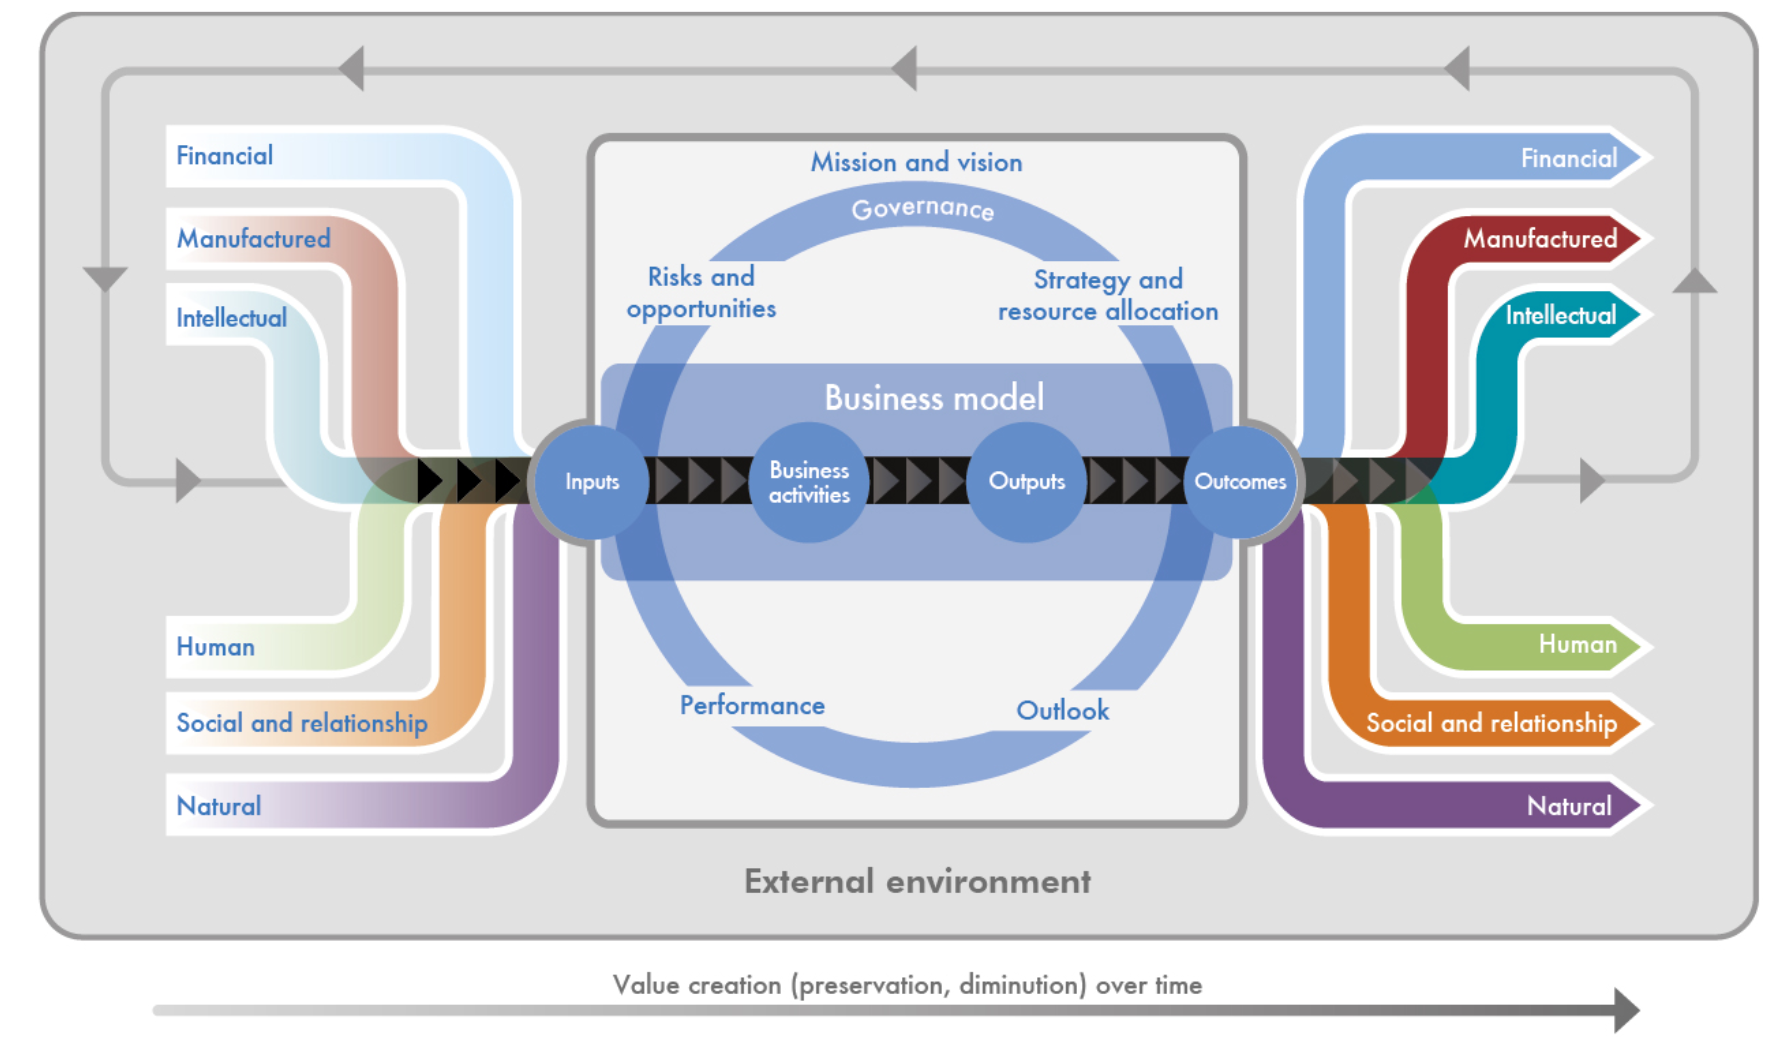
\includegraphics[width=0.8\linewidth]{img/IIRC_value_creation_process}
	\caption[The value creation process of the IIRC framework]{The value creation process of the IIRC framework\footnotemark}
	\label{fig:iircvaluecreationprocess}
\end{figure}
\footnotetext{\href{https://integratedreporting.org/wp-content/uploads/2013/12/13-12-08-THE-INTERNATIONAL-IR-FRAMEWORK-2-1.pdf}{The International \textless IR\textgreater Framework}}

\begin{figure}[H]
	\centering
	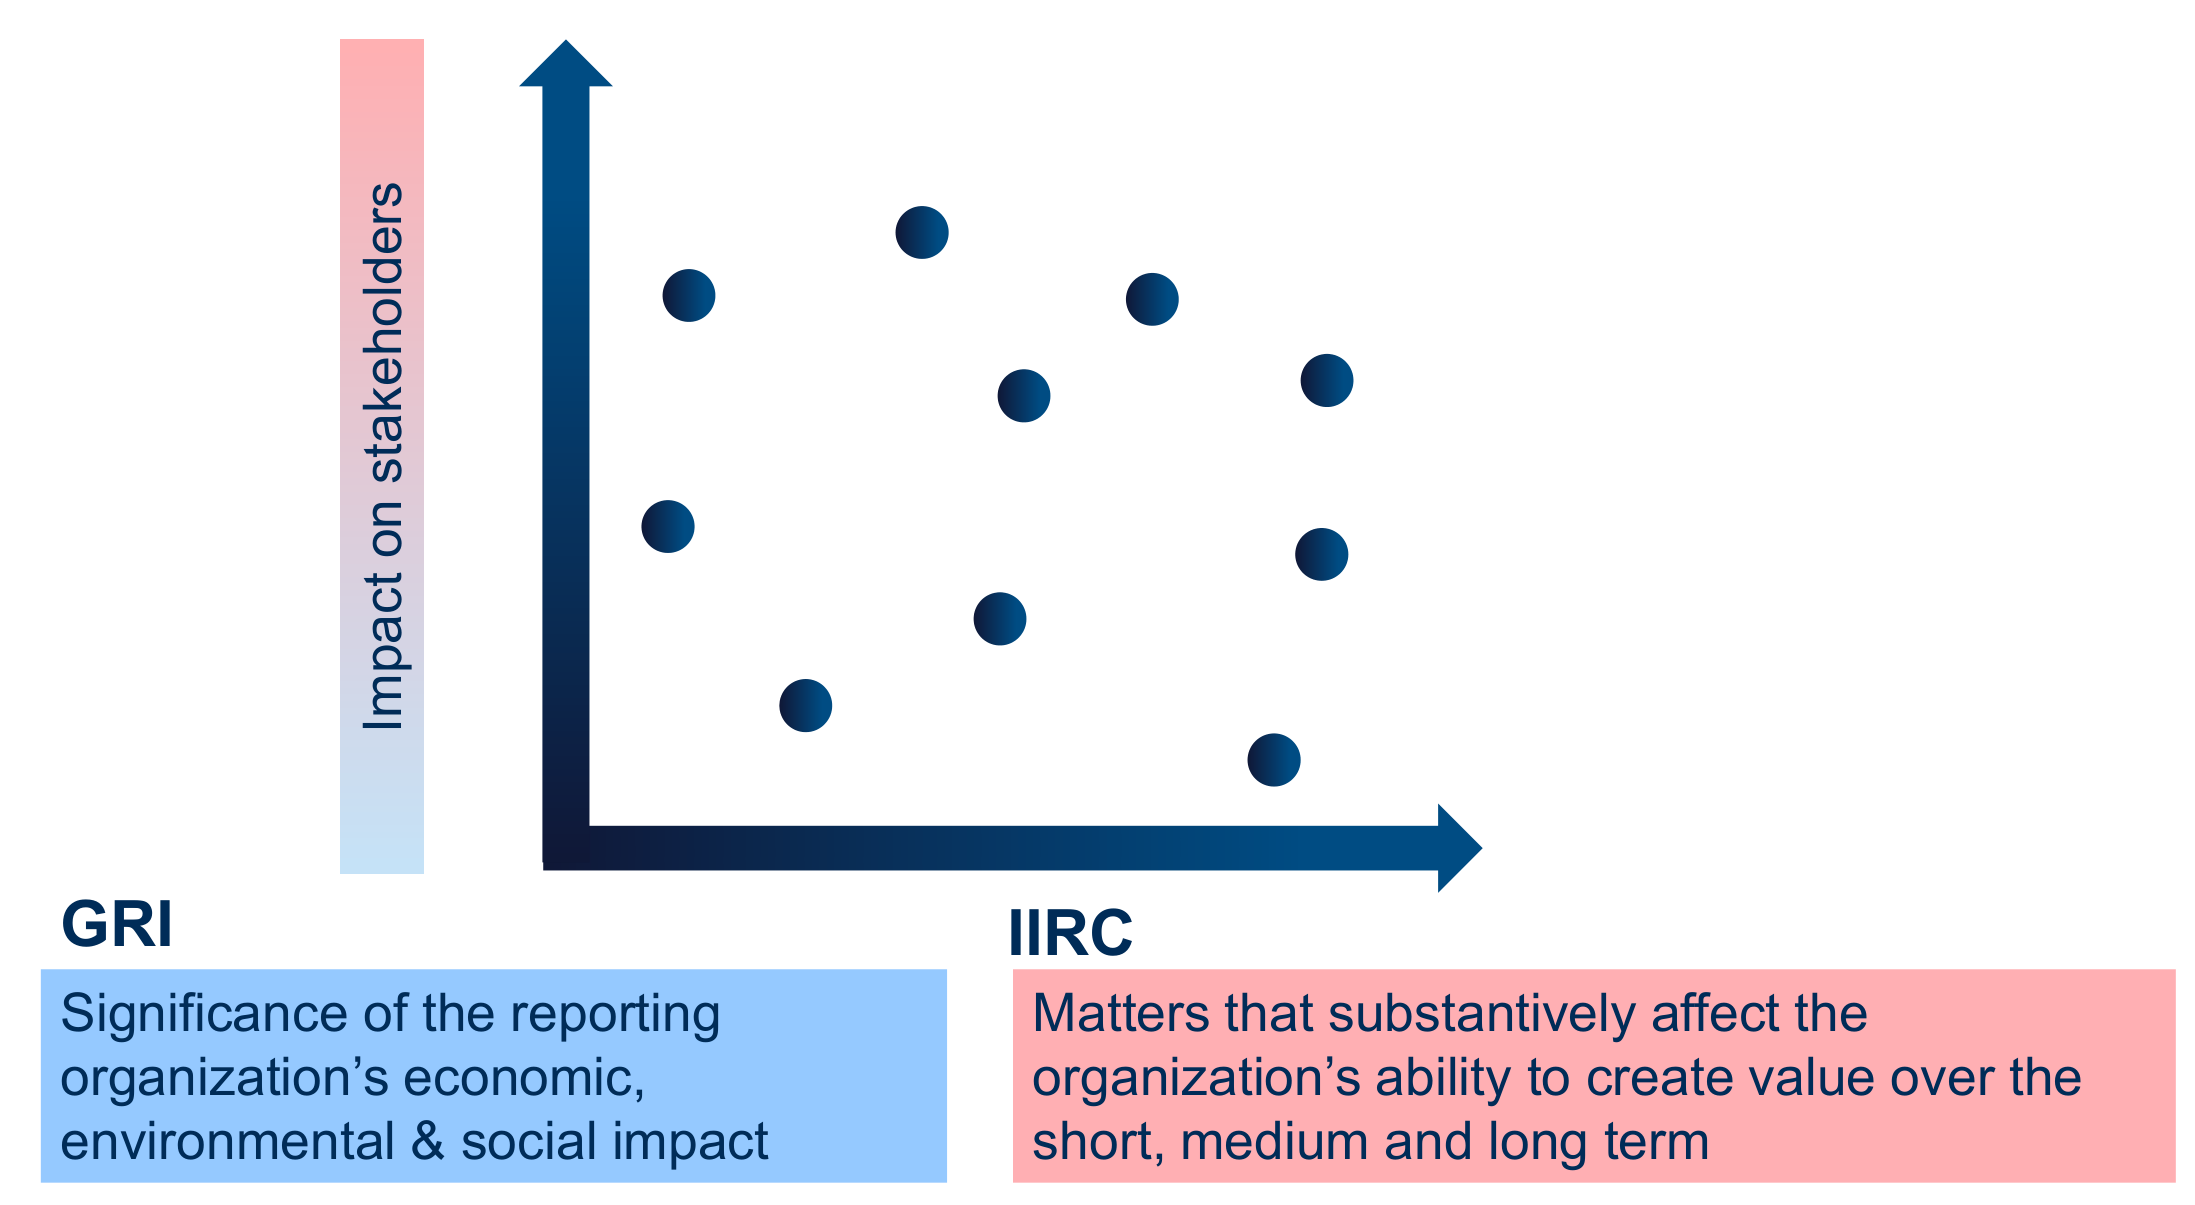
\includegraphics[width=0.8\linewidth]{img/comparison_IIRC_GRI}
	\caption{Comparison between reporting and materiality between the GRI and IIRC}
	\label{fig:comparisoniircgri}
\end{figure}

%TODO Check if formatting is still fine
\clearpage
\subsection{EU Directive on Non-Financial Reporting}
Financial and non-financial reporting provides shareholders and other stakeholders with a meaningful, comprehensive view of the position and performance of companies. Large public-interest entities designated by EU member states with more than
five-hundred employees should disclose relevant and useful information on their policies, main risks and outcomes in their management report, relating to at least
\begin{itemize}[nosep]
	\item environmental matters
	\item social and employee aspects
	\item respect for human rights
	\item anticorruption and bribery issues
	\item diversity in their board of directors
\end{itemize}
There is significant flexibility for companies to disclose relevant information (including reporting in a separate report), as well as they may rely on international, European or national guidelines.

\subsubsection{United Nation Global Compact (UNGC)}
The aim and vision of the UN Global Compact is to mobilise a global movement of sustainable companies and stakeholders to create a world everybody can live in.

To achieve this, the UNGC supports companies to
\begin{itemize}
	\item Do business responsibly by aligning their strategies and operations with Ten Principles\footnote{\href{https://www.unglobalcompact.org/what-is-gc/mission/principles}{UNGC Principles}} on human rights, labour, environment and anti-corruption
	\item Take strategic actions to advance broader societal goals, such as the UN Sustainable Development Goals\footnote{\href{https://www.unglobalcompact.org/what-is-gc/our-work/sustainable-development/sdgs}{The Sustainable Development Goals}}, with an emphasis on collaboration and innovation
\end{itemize}

\paragraph{The Ten Principles}
\begin{itemize}[leftmargin=*, label=, noitemsep]
	\item \textbf{Human Rights}
	\begin{itemize}[label=$\bullet$]
		\item Principle 1: Businesses should support and respect the protection of internationally proclaimed human rights; and
		\item Principle 2: make sure that they are not complicit in human rights abuses.
	\end{itemize}
	\item \textbf{Labour}
	\begin{itemize}[label=$\bullet$]
		\item Principle 3: Businesses should uphold the freedom of association and the effective recognition of the right to collective bargaining;
		\item Principle 4: the elimination of all forms of forced and compulsory labour;
		\item Principle 5: the effective abolition of child labour; and
		\item Principle 6: the elimination of discrimination in respect of employment and occupation.
	\end{itemize}
	\item \textbf{Environment}
	\begin{itemize}[label=$\bullet$]
		\item Principle 7: Businesses should support a precautionary approach to environmental challenges;
		\item Principle 8: undertake initiatives to promote greater environmental responsibility; and
		\item Principle 9: encourage the development and diffusion of environmentally friendly technologies.
	\end{itemize}
	\item \textbf{Anti-Corruption}
	\begin{itemize}[label=$\bullet$]
		\item Principle 10: Businesses should work against corruption in all its forms, including extortion and bribery.
	\end{itemize}
\end{itemize}

\subsubsection{Global Real Estate Sustainability Benchmark (GRESB)}
Members have to fill out a survey every year. This survey includes performance measures and indicators the companies have to report on. Subsequently, the survey is analysed by the GRESB committee. The company receives feedback and results, and for industries and regions, the GRESB provides a benchmark study.

\subsubsection{Principles for Responsible Investment (PRI)}
PRI reporting is the largest global
reporting project on responsible investment. It was developed with investors, for investors. Signatories are required to report on their responsible investment activities annually.

\begin{figure}[H]
	\centering
	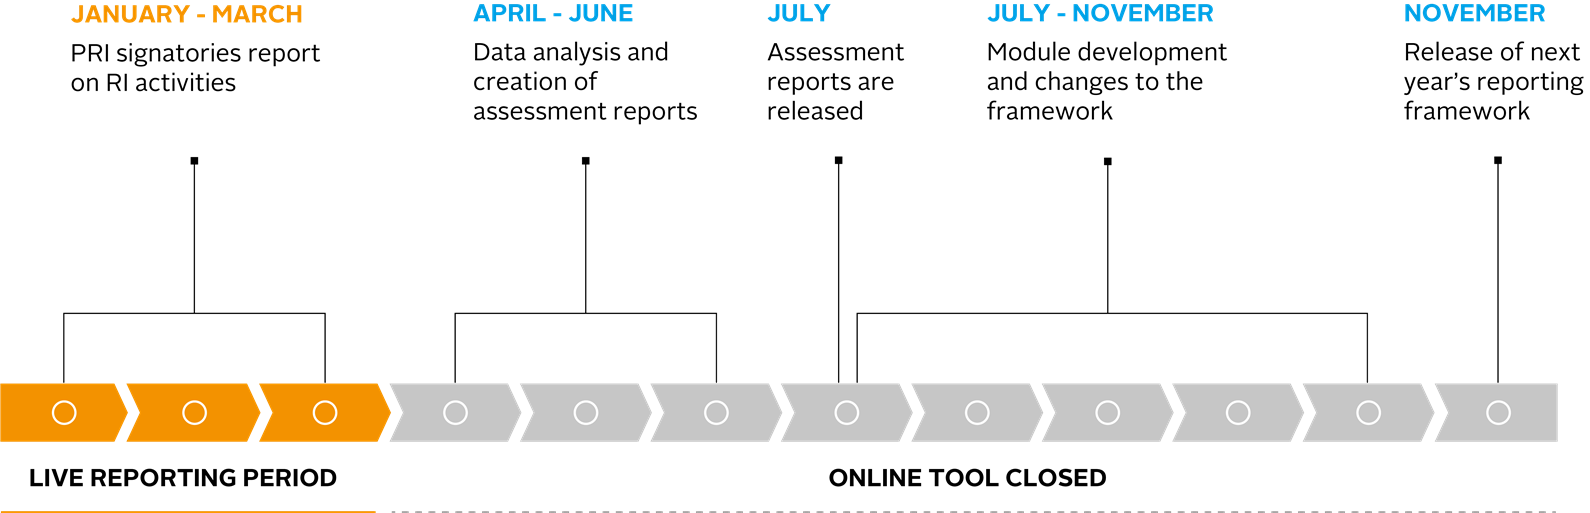
\includegraphics[width=0.8\linewidth]{img/PRI_reporting_process}
	\caption{PRI reporting process}
	\label{fig:prireportingprocess}
\end{figure}

\section{Corporate Responsibility Controlling}
Controlling is needed, as otherwise
\begin{quote}
	\textquotedblleft If it‘s not counted, it won‘t be noticed.\textquotedblright\\
	\hspace*{1em} - Alex MacGillivray, Simon Zadek
\end{quote}
\begin{itemize}
	\item The status of the company on the topic should be assessed and possibly compared with other companies (\textbf{benchmarking})
	\item The performance on corporate responsibility topics should be specifically controlled with targets and action plans (\textbf{controlling})
	\item The development of performance regarding the set targets should be tracked (\textbf{controlling})
	\item The status and development of performance on the topic should be communicated externally (\textbf{reporting})
\end{itemize}

\subsection{Added Value of Reporting and Benchmarking}
\paragraph{Reporting}
\begin{itemize}
	\item Creating a basis for reporting and communicating corporate responsibility issues internally and externally;
	\item Demonstrating to external stakeholders the extent to which the objectives have been met and that the success of corporate responsibility management is regularly reviewed, with measures taken when necessary.
\end{itemize}

\paragraph{Benchmarking}
\begin{itemize}
	\item Assessing the state and success of the company's corporate responsibility management and comparing it to other companies
\end{itemize}

\paragraph{Controlling}
\begin{itemize}
	\item Determining to what extent the strategy for corporate responsibility issues has been implemented;
	\item Determining to what extent the objectives have been achieved;
	\item Reviewing strategic and operational objectives as to their usefulness and revising them, if appropriate;
	\item Tracking the development of corporate responsibility performance over time;
	\item Questioning assumptions or actions related to corporate responsibility issues;
	\item Planning and controlling resources for corporate responsibility management better (learning effect);
	\item Visualizing and analysing relationships between causes and effects.
\end{itemize}

\subsubsection{Reasons for Deviations}
\begin{itemize}
	\item \textbf{Unrealistic Goals}\\ Goals that (a) are not based on experience or are not set by industry experts, and (b) are based on unrealistic assumptions
	\item \textbf{Poor Planning of Measures}\\ Courses of action unlikely to achieve the desired improvement in performance (that is on account of incorrect information about the relationship between cause and effect)
	\item \textbf{Poor Implementation}\\ Failure to implement suitable measures (that is owing to improper resources, unclear responsibilities, wrong incentives, trade-offs, or lack of expertise on the part of those responsible)
	\item \textbf{Unforeseen External and Internal Influences}\\ Examples of \textbf{external} influences include natural disasters, government regulatory measures, or crises related to corporate responsibility issues (combined with unexpected public attention towards the company)\\ Examples of \textbf{internal} influences include corporate reorganization
	\item \textbf{Deliberate Misconduct, Deception, Manipulation}\\ Conduct intended to sabotage the achievement of objectives or the effectiveness of measures
	\item \textbf{Unfavourable Conditions}\\ Examples include a lack of commitment by managers to achieving set objectives; a corporate culture that is opposed to the achievement of targets
\end{itemize}

%TODO Check if formatting is still fine
\clearpage
\subsubsection{Functions of Top Level Evaluation}
\begin{itemize}
	\item \textbf{Maintain What Works}\\ Analyse what works well and why; make sure it stays that way
	\item \textbf{Improve What Doesn't Work}\\ Analyse what does not work so well and why; identify obstacles and barriers, and initiate changes
	\item \textbf{Review Objectives}\\ Revisit original objectives and, where appropriate, take corrective action and set new goals
	\item \textbf{Ensure the Support of Senior Management}\\ The commitment of executives is crucial; for this reason, their involvement in major decision-making is essential
	\item \textbf{Track Current Trends}\\ Senior management should be familiar with major developments both within and outside the company
	\item \textbf{Provide Resources}\\ Decisions must be taken at an executive level to ensure the necessary resources for further development are made available
	\item \textbf{Celebrate Achievements}\\ An assessment of a past period is an excellent opportunity to celebrate achievements with awards, prizes, or certificates, preferably involving all stakeholders
\end{itemize}

\clearpage
%%% BIBLIOGRAPHY %%%

\printbibliography

\end{document}
